%% TOMPECS manuscript -- ACM Transactions on Modeling and Performance Evaluation of Computing Systems.
%% Template: acmart, format `acmsmall` (the acmart guide lists TOMPECS under acmsmall).
%% `review` is the submission/review-copy option; remove it for the camera-ready version.
%% Review type (single- or double-blind) is NOT confirmed: if double-blind, add the `anonymous`
%% option and wrap the acknowledgments in \begin{anonsuppress}...\end{anonsuppress}.
%% Built from the earlier ACL-style sections by tools/assemble.py, then restructured on 2026-10-29
%% (methodology / setup / results / discussion / related work / conclusion); see MAPPING.md.
\documentclass[acmsmall,review]{acmart}

\usepackage{multirow}
\usepackage{xspace}
\usepackage{amssymb}
\usepackage{tikz}
\usetikzlibrary{arrows.meta,positioning,calc}
%% Tick and cross for the prompt-variant table.
\newcommand{\cmark}{\checkmark}
\newcommand{\xmark}{$\times$}
\newcommand{\tzi}[1]{\textcolor{red}{FIX: #1}\xspace}
%% Marks a statement that still needs evidence or an author decision. Remove every use before submitting.
\newcommand{\needcheck}[1]{\textcolor{blue}{[CHECK: #1]}\xspace}

%% --- journal metadata (volume, number, article number, DOI and dates are assigned by ACM) ---
\acmJournal{TOMPECS}
%\acmVolume{}
%\acmNumber{}
%\acmArticle{}
%\acmYear{2026}
%\acmMonth{}
%\acmDOI{}

\begin{document}

\title{Prompting for Performance: Profile-Guided LLM Optimization of Real GPU Applications}

%% TODO: real author details. TOMPECS requires an ORCID for every submitting author.
\author{First Author}
\orcid{0000-0000-0000-0000}
\affiliation{%
  \institution{Institution}
  \city{City}
  \country{Country}}
\email{email@domain}

\author{Second Author}
\orcid{0000-0000-0000-0000}
\affiliation{%
  \institution{Institution}
  \city{City}
  \country{Country}}
\email{email@domain}

\renewcommand{\shortauthors}{First Author and Second Author}

\begin{abstract}
% EDIT (2026-10-29): rewritten to the author's outline ("showing how prompt design affects the
% outcome ... we show 1) the impact of guardrails 2) the importance of profiling data 3) ..."). Every
% number is one already reported in the body; the per-variant first-attempt counts are read off
% Table~\ref{tab:ablation}.
We present an empirical study of how prompt design affects what a large language model does when it
is asked to make GPU code faster, and of how far the gains it finds survive on production scientific
applications. Our framework, OPTIMAS, closes the loop from profiling to prompting, generation, build,
correctness check and timed measurement, with up to three repair iterations driven by compiler and
runtime feedback. We vary the prompt one component at a time and measure the outcome on HeCBench
kernels and on two production applications, AutoDock-GPU and Cholla, each checked against its own
scientific output. We show (1) the impact of guardrails: which instructions the prompt carries decides
how often a model returns a valid candidate at the first attempt (between $8$ and $11$ of $12$ runs,
depending on which component is removed) and how slow its worst result is; and without an explicit
semantic-preservation rule both models ``optimize'' a benchmark by deleting the computation it exists
to measure, reporting $1504\times$ and $2809\times$ while the benchmark's own check still passes;
(2) the importance of profiling data: removing it from an otherwise identical prompt costs
$7.7$--$11.5\%$ on a 21k-line application, while on single-kernel benchmarks it moves individual
results in both directions with no net gain; (3) the limits of interpreting that data for the model:
converting profiler metrics into a checklist of named remedies produces both our largest gain
($1.00\times \to 1.38\times$) and our largest loss ($0.84\times \to 0.35\times$), so its effect is a
wider spread of outcomes rather than a better average; and (4) what the models can and cannot do:
they reliably find local, exact transformations---on Cholla all four outputs under the baseline
prompt ($1.48$--$1.58\times$) beat our hand-tuned reference ($1.47\times$)---and reliably miss
cross-cutting restructuring, leaving unfound on AutoDock-GPU the reduction fusion that is worth
$1.53\times$ by hand. We also report the problems that appear only on real code and the measurement
practice needed to report any of this credibly on shared GPUs.

% ---------------------------------------------------------------------------
% ORIGINAL ABSTRACT (kept for reference). It describes three prompt designs
% (loose / constrained / agentic) and a one-shot agentic result; the version above
% was rewritten to match the experiments currently in the paper (six-variant
% ablation, semantic-preservation constraint, two applications, profile-data
% ablation). Restore or merge if the agentic-prompt experiment is added.
%
% We present an empirical study of how progressively adding task-specific guardrails to prompts
% impacts large language models' ability to generate code optimization suggestions for HPC workloads.
% Across three prompt designs, we observe that tighter guardrails systematically shift model behavior
% from aggressive but low-utility transformations toward conservative, high-utility optimizations that
% compile, preserve numerical correctness, and yield measurable performance gains. The first prompt,
% which loosely describes the optimization task, produces many syntactically plausible but
% non-compiling or numerically incorrect suggestions and often requires up to ten
% optimization-feedback iterations to reach a viable configuration. The second prompt introduces
% explicit constraints on correctness, safety, and resource usage, reducing over-aggressive
% transformations and increasing the fraction of optimizations that lead to positive speedups without
% degrading numerical accuracy. Finally, our most constrained "agentic" prompt instantiates a
% closed-loop optimization routine in which the LLM autonomously proposes an optimization, checks
% compilation and numerical correctness against a reference, and revises its plan before returning a
% single final suggestion, achieving one-shot successful optimization on our benchmarks. We evaluate
% these prompts on diverse HPC kernels and systems, and we quantify their effects along three axes:
% performance gain, correctness, and optimization aggressiveness (e.g., code churn, magnitude of
% configuration change). Our results show that guardrail design is not merely a safety or policy
% concern, but a central lever for turning general-purpose code LLMs into reliable performance
% co-designers for scientific computing.
% ---------------------------------------------------------------------------

\end{abstract}

%% TODO(verify): these CCS concepts were written from memory and are NOT checked against the ACM
%% classification. Regenerate the CCSXML block and \ccsdesc lines with the tool at
%% https://dl.acm.org/ccs before submitting; a wrong identifier gives wrong indexing metadata.
\begin{CCSXML}
<ccs2012>
 <concept>
  <concept_id>10002944.10011123.10011674</concept_id>
  <concept_desc>General and reference~Performance</concept_desc>
  <concept_significance>500</concept_significance>
 </concept>
 <concept>
  <concept_id>10002944.10011123.10010912</concept_id>
  <concept_desc>General and reference~Empirical studies</concept_desc>
  <concept_significance>300</concept_significance>
 </concept>
 <concept>
  <concept_id>10011007.10010940.10011003.10011002</concept_id>
  <concept_desc>Software and its engineering~Software performance</concept_desc>
  <concept_significance>300</concept_significance>
 </concept>
 <concept>
  <concept_id>10011007.10011006.10011041</concept_id>
  <concept_desc>Software and its engineering~Compilers</concept_desc>
  <concept_significance>100</concept_significance>
 </concept>
 <concept>
  <concept_id>10010520.10010521.10010528</concept_id>
  <concept_desc>Computer systems organization~Parallel architectures</concept_desc>
  <concept_significance>100</concept_significance>
 </concept>
</ccs2012>
\end{CCSXML}

\ccsdesc[500]{General and reference~Performance}
\ccsdesc[300]{General and reference~Empirical studies}
\ccsdesc[300]{Software and its engineering~Software performance}
\ccsdesc[100]{Software and its engineering~Compilers}
\ccsdesc[100]{Computer systems organization~Parallel architectures}

\keywords{LLM-driven code optimization, GPU performance engineering, profile-guided prompting,
performance evaluation methodology, benchmark validity, measurement on shared systems}

\maketitle

\section{Introduction}
\label{sec:intro}
GPU performance engineering is expert work. Getting a kernel to run faster requires reasoning about the
memory hierarchy, warp scheduling, occupancy and instruction-level behaviour at the same time, and
expert tuners routinely spend weeks on a single kernel. Large language models can attempt the same edit
in seconds, which raises an obvious question: how much of that expertise can be supplied through the
prompt, and how much of the resulting speedup survives contact with a real application?

Existing code benchmarks do not answer this. HumanEval-style suites \cite{chen2021codex} and
repository-level issue resolution \cite{jimenez2024swebench} score functional correctness, not
execution time, and recent GPU-specific benchmarks \cite{ouyang2025kernelbench,nichols2024parallel}
evaluate standalone kernels written from a reference implementation rather than edits to code that a
scientific application already depends on. Meanwhile, the first thing a human expert looks at---profiler
output---is exactly the kind of context an LLM never sees by default.

This paper studies an end-to-end loop that closes that gap: profile the application, summarize the
profile into the prompt, ask the model for an optimized version of one source file, build it, verify it
against the application's own notion of correctness, measure it, and feed failures back for a bounded
number of repair iterations. Within this loop we treat the prompt as the object of study.
% NEW (written for the TOMPECS version; not in the original paper)
Because the loop's output is a measured execution time, the study is as much about how such systems
must be \emph{evaluated} as about how they should be prompted. We organize it around five research
questions:
\begin{description}\itemsep2pt
\item[RQ1] Which components of the prompt matter, and how reliably? (Section~\ref{sec:prompts})
\item[RQ2] Can speedups reported on benchmarks be trusted, and what does a model do when the
  benchmark's own scaffolding can be deleted? (Section~\ref{sec:intent})
\item[RQ3] Do conclusions drawn on single-kernel benchmarks transfer to the production applications
  those kernels represent? (Section~\ref{sec:realapps})
\item[RQ4] What is profiling evidence worth, supplied raw and supplied interpreted?
  (Section~\ref{sec:evidence})
\item[RQ5] What measurement and validation practice is needed to report any of this credibly on shared
  hardware? (Sections~\ref{sec:method}, \ref{sec:pitfalls} and~\ref{sec:limits})
\end{description}
Our contributions are:

\begin{itemize}\itemsep2pt
\item \textbf{A prompt-component ablation} over six variants, two models and six HeCBench kernels
  (Sections~\ref{sec:ablation}--\ref{sec:results}), showing that prompt components are not equally
  important: stripping the instructions (\texttt{minimal}) gives the slowest valid result more
  often than any other variant, while an explicit reasoning step (\texttt{cot}) never does, although
  it does not prevent outright failures.
\item \textbf{A semantic-preservation constraint} that suppresses benchmark gaming
  (Section~\ref{sec:intent}). Without it, both models delete the very computation a benchmark exists to
  measure and report speedups of $1504\times$ and $2809\times$ while output and the built-in
  verification remain unchanged; with it, both return honest results. We also report the detection rule
  we use, since neither output comparison nor the benchmark's own check can catch this class of edit.
\item \textbf{An end-to-end evaluation on three production applications}---AutoDock-GPU, LAMMPS and
  Cholla (Section~\ref{sec:realapps})---with per-application correctness gates that we validate by
  fault injection, and interleaved measurement on shared GPUs. The best model output reaches
  $1.571\times$ on Cholla, beating our expert hand-tuned reference, while on AutoDock-GPU no model or
  prompt found the restructuring that is worth $1.532\times$ by hand.
\item \textbf{A profile-data ablation} (Section~\ref{sec:profabl}) that isolates the contribution of
  PC-sampling and roofline data by removing it from an otherwise identical prompt. Profiling data is
  worth $7.7$--$11.5\%$ on the large application and nothing measurable on single-kernel benchmarks,
  which suggests its value scales with how hard the bottleneck is to locate from source alone.
\item \textbf{A measurement of what happens when profiling data is made prescriptive}
  (Section~\ref{sec:guidvar}). Converting metrics into a checklist of named remedies produces both our
  largest gain ($1.04\times \to 1.38\times$) and our largest loss ($7.84\times \to 1.08\times$, where the
  checklist displaced a restructuring the model had found unaided), at repetition spreads below $5\%$.
  Interpretation widens the distribution of outcomes rather than shifting its centre, which a mean
  speedup hides.
\item \textbf{A set of failure modes specific to real code} (Section~\ref{sec:defects}), including compilation-context blindness
  (the model cannot see that its file is textually included elsewhere, or that ten call sites depend on
  a signature), applications whose error handling discards the diagnostic the repair loop needs, and
  measurement pitfalls on shared machines that silently invalidate results.
\end{itemize}

Taken together, the results argue that prompt design is a first-order lever for turning general-purpose
code models into usable performance tools---but also that conclusions drawn on single-kernel benchmarks
do not automatically transfer to the applications those kernels are meant to represent.

% NEW (written for the TOMPECS version; not in the original paper)
\paragraph{Organization.}
Section~\ref{sec:relatedwork} places the work in the literature and Section~\ref{sec:subject}
describes the optimization pipeline under study. Section~\ref{sec:method} states the workloads,
platforms, correctness validation and measurement protocol on which every later number depends.
Sections~\ref{sec:prompts}--\ref{sec:evidence} report the four studies behind RQ1--RQ4,
Section~\ref{sec:pitfalls} collects the evaluation pitfalls they exposed, Section~\ref{sec:limits}
states the threats to validity, and Section~\ref{sec:conclusions} concludes.

\section{Methodology}
\label{sec:method}
% EDIT (2026-10-29): new section built from the old Sections 3 (pipeline, profiling data, prompt
% structure), 5.1 (prompt variants), 6.2 (constraint text), 4.3--4.5 (correctness, timing, reporting
% conventions), 7.2--7.3 (gates, application timing) and the "Arms"/"Setup" paragraphs of 8.1 and 8.2,
% following the reviewer's requested structure. The variant descriptions were re-derived from the
% saved prompts (diffs of src/results/atan2-codex-gpt5-<variant>/*prompt_1.txt against the cot prompt)
% and correct two statements of the earlier text: no_constraints removes only the six rules written
% as "Do NOT", and minimal keeps the hardware guidance and the entry-point guardrails.
This section describes the system under study---the optimization loop, the profiling data it can
place in the prompt, and the prompt itself---and then the prompt variants, the correctness checks and
the measurement protocol on which every result depends.

\subsection{The Optimization Loop}
\label{sec:subject}
The framework takes a source file, a build-and-run script and the profile of the program, and closes
the loop shown in Figure~\ref{fig:pipeline}: \emph{profile $\rightarrow$ summarize $\rightarrow$ prompt
$\rightarrow$ generate $\rightarrow$ build $\rightarrow$ verify $\rightarrow$ measure}, with bounded
repair. Profiling happens once, before the loop. The prompt carries the source file, the profile
summaries and the instructions described below; the model answers with a complete replacement for the
file. That file replaces the original in a private copy of the program tree, so the build, the callers
and the input data are those of the real program. The build-and-run script then compiles the program,
runs it, and applies its correctness check. If compilation fails, the program crashes, or the check
prints a failure, the loop summarizes the build log (at most $80$ lines), assembles a repair prompt
from the original source, the rejected candidate and that summary, and asks the model again; a repair
that returns the candidate unchanged is rejected and requested once more. We allow three iterations
before recording the run as a failure. When a candidate builds and passes, the loop records its
in-loop execution time, the average of ten runs of the binary. That number serves the loop only; the
timings reported in this paper come from a separate interleaved measurement pass
(Section~\ref{sec:timing}).

\begin{figure}[t]
\centering
\resizebox{\textwidth}{!}{%% Workflow of the optimization loop (Figure 1). NEW (2026-10-29), drawn from src/opal_cli_codex.py:
%% prompt -> LLM -> candidate -> build+run script (build, run, built-in check or gate) -> on error,
%% summarized log -> repair prompt -> LLM, at most three iterations -> in-loop 10-run average.
%% Profiling (two Nsight Compute passes) runs before the loop; the reported timings come from a
%% separate interleaved pass. Needs \usetikzlibrary{arrows.meta,positioning,calc} (main.tex).
%% Layout: row 1 profile..candidate; row 2 (right to left) build, verify, measure, timing pass;
%% row 3 the repair step under build. No arrow crosses a node; the loop back to the model runs
%% above row 1. NOT compiled yet (no LaTeX here): if a build fails, check this file first.
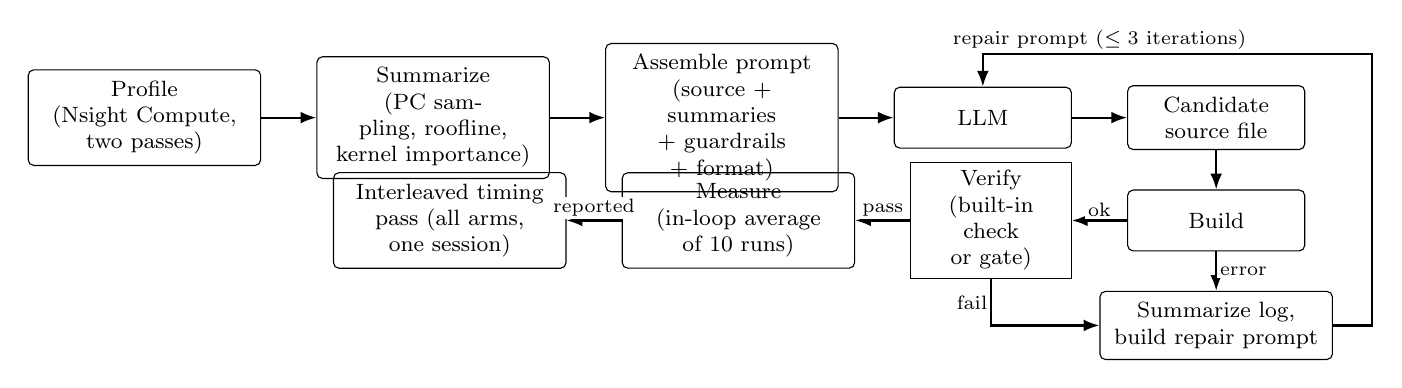
\begin{tikzpicture}[
  font=\footnotesize,
  box/.style={draw, rounded corners=2pt, align=center, minimum height=2.2em, inner sep=4pt,
              text width=5.6em},
  wide/.style={box, text width=7.6em},
  dec/.style={draw, align=center, minimum height=2.2em, inner sep=3pt, text width=5.2em},
  arr/.style={-{Latex[length=2mm]}, thick},
  lab/.style={font=\scriptsize, fill=white, inner sep=1pt},
  node distance=5mm and 7mm
]
  % row 1: before the loop, and the generation step
  \node[wide] (prof)   {Profile\\(Nsight Compute,\\two passes)};
  \node[wide, right=of prof] (summ) {Summarize\\(PC sampling, roofline,\\kernel importance)};
  \node[wide, right=of summ] (prompt) {Assemble prompt\\(source + summaries\\+ guardrails + format)};
  \node[box,  right=of prompt] (llm) {LLM};
  \node[box,  right=of llm] (cand) {Candidate\\source file};
  % row 2: build, verify, measure, and the separate timing pass
  \node[box,  below=of cand] (build) {Build};
  \node[dec,  left=of build] (verify) {Verify\\(built-in check\\or gate)};
  \node[wide, left=of verify] (measure) {Measure\\(in-loop average\\of 10 runs)};
  \node[wide, left=of measure] (report) {Interleaved timing\\pass (all arms,\\one session)};
  % row 3: repair
  \node[wide, below=of build] (repair) {Summarize log,\\build repair prompt};

  \draw[arr] (prof) -- (summ);
  \draw[arr] (summ) -- (prompt);
  \draw[arr] (prompt) -- (llm);
  \draw[arr] (llm) -- (cand);
  \draw[arr] (cand) -- (build);
  \draw[arr] (build) -- node[lab, above] {ok} (verify);
  \draw[arr] (verify) -- node[lab, above] {pass} (measure);
  \draw[arr] (measure) -- node[lab, above] {reported} (report);
  \draw[arr] (build) -- node[lab, right] {error} (repair);
  \draw[arr] (verify.south) |- node[lab, pos=0.25, left] {fail} (repair.west);
  \draw[arr] (repair.east) -- ++(5mm,0) |- ($(cand.north)+(0,4mm)$)
             -| node[lab, pos=0.25, above] {repair prompt ($\le 3$ iterations)} (llm.north);
\end{tikzpicture}
}
\caption{The optimization loop. Profiling and summarization run once; the prompt, model, build and
  verification steps form the repair loop, bounded at three iterations. The in-loop time is used only
  to record the run; every timing reported in this paper comes from the separate interleaved pass of
  Section~\ref{sec:timing}.}
\label{fig:pipeline}
\end{figure}

\subsection{Profiling Data}
\label{sec:profdata}
% EDIT (2026-10-29): more context on what each kind of data is, asked for in review.
The profile comes from Nsight Compute, NVIDIA's kernel profiler, in two passes over the program: an
uncapped pass that records every kernel launch and gives true launch counts and per-launch durations,
and a capped \texttt{-{}-set full} pass over a bounded number of launches that collects the detailed
metric pages. From the two reports we derive three kinds of prompt context, each rendered as a short
text or JSON summary:
\begin{itemize}\itemsep2pt
  \item \textbf{PC sampling} (\texttt{-{}-page source}). The profiler periodically samples the program
    counter of running warps and records, for each sample, whether the warp was stalled and why (waiting
    on memory, on a math unit, on a barrier, and so on). Aggregated per source line, this says which
    lines the kernel spends its time on and what those lines are waiting for. The summary lists the
    lines with the highest stall ratios, each with its source text and its stall reasons, so that the
    model can refer to them by line number.
  \item \textbf{Roofline} (\texttt{-{}-page details}). For each kernel, the achieved DRAM and compute
    throughput relative to the device's peaks, which says whether the kernel is bound by memory
    bandwidth, by arithmetic throughput, or by neither (latency-bound), together with the analysis rules
    that Nsight Compute itself reports for the kernel.
  \item \textbf{Kernel importance}. The aggregate cost of each kernel (launch count $\times$ per-launch
    time), used to rank which kernel is worth editing at all. For the single-kernel benchmarks this is
    trivial; for the applications it is what selects the target file.
\end{itemize}
The arms that remove or extend this evidence are defined with the prompt variants below.

\subsection{Prompt Structure}
\label{sec:promptstructure}
% EDIT (2026-10-29): the regions are now listed in the order they appear in the prompt, with an excerpt
% of each (Table~\ref{tab:prompt}), taken from the saved prompt
% src/results/atan2-codex-gpt5-cot/atan2_pc+rl_gpt5_cot_prompt_1.txt.
Table~\ref{tab:prompt} shows the full prompt region by region, with the text of each region as sent.
A one-line persona is sent as the system message. The user message then carries, in order: the
numbered source file; the profile summaries; a hardware-guidance paragraph naming the Hopper features
to target; five entry-point guardrails that protect the program's \texttt{main} and its linkage; and
the instruction block. The instruction block states the task and requires a correctness argument
(preconditions, postconditions, loop invariants and a proof that the transformation preserves them),
and then gives nineteen numbered rules: six prohibitions written as ``Do NOT'' (no new top-level
symbols, no wrapper helpers, no larger shared-memory footprint, and three entry-point rules), a set of
working rules (use the profile's line references, make at least one substantive change, keep the code
unchanged and say so if none is justified, no line numbers, no renamed functions or changed
signatures), and the output format: the complete source in one fenced code block followed by two
structured lists, the optimizations applied and those considered but not applied.

\begin{table}[t]
\centering
\footnotesize
\caption{The prompt, region by region, with the text as sent (excerpts; $\langle\cdot\rangle$ marks
  generated content). The persona is the system message; everything else is the user message, in this
  order.}
\label{tab:prompt}
\begin{tabular}{@{}p{0.2\textwidth}p{0.76\textwidth}@{}}
\toprule
\textbf{Region} & \textbf{As sent} \\
\midrule
Persona (system message) & \texttt{You are an HPC performance optimization expert.} \\
Source file & \texttt{\# Begin Source Code} $\langle$the file, one numbered line per source line$\rangle$
  \texttt{\# End Source Code} \\
Profile summaries & \texttt{\# Begin Performance Analysis} $\langle$PC-sampling summary: for each hot
  line, its number, its source text and its stall reasons$\rangle$ $\langle$roofline summary$\rangle$
  \texttt{\# End Performance Analysis} \\
Hardware guidance & \texttt{Optimize specifically for NVIDIA H100 (Hopper) by targeting L2/cache reuse,
  HBM3 bandwidth, and Tensor Core throughput. Prioritize tiling and data locality: \ldots} \\
Entry-point guardrails & \texttt{1. The source already contains 1 main() definition(s). Preserve exactly
  that many main() definitions. 2. Do NOT add a new main(), duplicate main(), rename main(), \ldots} \\
Task and proof requirement & \texttt{Optimize the following HPC code for execution time. You must define
  mathematical preconditions and postconditions, provide explicit loop invariants to guarantee semantic
  equivalence, and provide a logical proof showing why the invariants remain unbroken \ldots} \\
Prohibitions & \texttt{9. Do NOT introduce any new helper functions, utility functions, macros,
  templates, classes, structs, global variables, or other new top-level symbols \ldots\
  11. Do NOT increase the total shared-memory footprint of any kernel \ldots} \\
Working rules & \texttt{12. Use the performance analysis reference number(s) to guide your changes.
  \ldots\ 15. When the performance data supports it, apply at least one substantive
  performance-motivated code change \ldots\ 16. If no safe substantive optimization can be justified
  \ldots, keep the code semantically unchanged and say so explicitly \ldots} \\
Output format and explanation & \texttt{17. Return: (a) the full source code including the optimized
  kernels inside {\textasciigrave\textasciigrave\textasciigrave} block (b) optimizations list = [\{'lines': [...], 'reason': '...'\}] (c)
  suggested\_but\_not\_applied list = [\{'lines': [...], 'reason': '...'\}]} \\
Step-by-step instruction (\texttt{cot} only) & \texttt{Think step by step about which bottlenecks to
  address and why before writing any code.} \\
\bottomrule
\end{tabular}
\end{table}

\subsection{Prompt Variants}
\label{sec:ablation}
To find out which parts of the prompt matter, the prompt-component study evaluates six variants, each
of which removes or adds exactly one region while leaving the source file and the profile summaries in
place. Table~\ref{tab:variants} shows which regions each variant carries. We describe them from the
least populated prompt to the most populated one; the effect of each is reported in
Section~\ref{sec:prompts}.

\begin{table}[t]
\centering
\footnotesize
\setlength{\tabcolsep}{4pt}
\caption{Prompt regions carried by each variant of the prompt-component study, from the least to the
  most populated. The persona, the source file, the profile summaries and the single-code-block output
  requirement are present in every variant. \cmark\ = present, \xmark\ = absent.}
\label{tab:variants}
\begin{tabular}{@{}lcccccc@{}}
\toprule
\textbf{Region} & \texttt{minimal} & \texttt{no\_role} & \texttt{no\_constraints} & \texttt{no\_proof}
  & \texttt{no\_explanation} & \texttt{cot} \\
\midrule
Hardware guidance            & \cmark & \xmark & \cmark & \cmark & \cmark & \cmark \\
Entry-point guardrails       & \cmark & \cmark & 2 of 5 & \cmark & \cmark & \cmark \\
Proof requirement            & \xmark & \cmark & \cmark & \xmark & \cmark & \cmark \\
Prohibitions (``Do NOT'')    & \xmark & \cmark & \xmark & \cmark & \cmark & \cmark \\
Working rules                & \xmark & \cmark & \cmark & \cmark & \cmark & \cmark \\
Explanation lists            & \xmark & \cmark & \cmark & \cmark & \xmark & \cmark \\
Step-by-step instruction     & \xmark & \xmark & \xmark & \xmark & \xmark & \cmark \\
\bottomrule
\end{tabular}
\end{table}

\paragraph{Minimal (\texttt{minimal}).}
The whole instruction block---task statement, proof requirement, the nineteen rules and the output
format---is replaced by one sentence: \textit{``Optimize the following CUDA code for execution time.
Return the complete optimized source in a single \texttt{cpp} block.''} The source, the profile
summaries, the hardware guidance and the entry-point guardrails remain, so \texttt{minimal} isolates
the value of the \emph{instructions}; removing the evidence instead is the separate profile-data
ablation (\texttt{code\_only}, below).

\paragraph{No Role (\texttt{no\_role}).}
Removes the hardware-guidance paragraph, which tells the model which Hopper features to target (cache
reuse, asynchronous copies, Tensor Cores, occupancy, warp efficiency). The one-line persona is a system
message and stays in every variant.

\paragraph{No Constraints (\texttt{no\_constraints}).}
Removes the six rules written as prohibitions: no new helper functions, macros, templates or other
top-level symbols; no wrapper load helpers; no larger shared-memory footprint; no second entry point;
no wrapper executables; and no renaming of externally referenced functions. The remaining rules
(including ``do not change any function signatures'' and ``do not rename or duplicate any kernel'')
stay, so the variant frees the model to add code around the existing kernels rather than to change
their interface.

\paragraph{No Proof (\texttt{no\_proof}).}
Removes the sentence that requires preconditions, postconditions, loop invariants and a proof of
semantic equivalence. The model may then apply a transformation without having to argue that it
preserves the computation.

\paragraph{No Explanation (\texttt{no\_explanation}).}
Removes the two structured lists from the required output---the optimizations applied and those
considered but not applied---and asks for the code alone. Having to name and justify each change is a
form of implicit reasoning, and the lists are also the record from which we reconstruct \emph{why} a
run behaved as it did.

\paragraph{Chain of Thought (\texttt{cot}).}
Unlike the others, \texttt{cot} adds a region: the instruction \textit{``Think step by step about which
bottlenecks to address and why before writing any code''} is prepended to the instruction block. It is
the most populated prompt in the study and, since the study has no separate full-prompt arm, the
closest thing to one.

\paragraph{Variants not evaluated.}
Two further variants are implemented but excluded from the measured grid. \texttt{no\_format} strips
the output-format requirement and asks only for optimized code; it perturbs the reliability of
automated code extraction rather than the quality of the optimization, which would confound the metric.
\texttt{no\_hardware} removes the hardware-guidance paragraph and the target-architecture line; in the
prompt format used here it removes the same paragraph as \texttt{no\_role}, so it is subsumed.

\paragraph{Variants used in the later experiments.}
Three prompts defined after the component study are used in Sections~\ref{sec:realapps}
to~\ref{sec:guidvar}:
\begin{itemize}\itemsep2pt
  \item \textbf{Baseline} is the full prompt of Table~\ref{tab:prompt} with PC-sampling and roofline
    summaries (\texttt{pcrl} in the profile-data ablation, where the name distinguishes it from the arm
    without data).
  \item \textbf{Structural} relaxes the prohibitions: it allows new kernels, helpers and templates,
    signature and launch-configuration changes, and shared-memory staging, under an explicit contract
    that the computation is preserved, and it adds two derived summaries, a per-kernel budget (launch
    count, aggregate time, DRAM and SM utilization, bound verdict) and an occupancy summary (achieved
    occupancy, waves per SM, and the resource that limits occupancy).
  \item \textbf{Diagnostics} is the structural prompt plus a bounded checklist of measured conditions
    and the transformation each one suggests. Each item is triggered by the kernel's own numbers
    (occupancy, DRAM and SM throughput, shared-memory use) and names a remedy, for example
    \textit{``Is a value read from and written back to global memory inside the innermost loop (an
    accumulator, counter or running sum)? \ldots\ Accumulate in a local variable and store once after
    the loop.''} It is our instance of profiling data made prescriptive.
    % Quoted from src/DiagnosticsSummarization.py, item (a).
  \item \textbf{Code only} (\texttt{code\_only}) is the baseline prompt without the profile summaries.
    Removing the summaries alone would bias the comparison, because four instruction sentences refer to
    the data---most importantly rule 16, \textit{``if no safe substantive optimization can be
    justified from the provided performance data, keep the code semantically unchanged''}, which would
    invite a no-op when no data is present. Those four sentences are reworded to refer to the model's
    own analysis of the source; the two prompts are otherwise byte-identical (verified: the diff is the
    removed block plus those four sentences).
\end{itemize}

\subsection{The Semantic-Preservation Constraint}
\label{sec:constraint}
% EDIT (2026-10-29): constraint text moved here from the old Section 6.2; the dates of the arms that
% carry it are from the saved prompts on the cluster (bincount-gpt5 2026-09-09: absent;
% bincount-gpt5-struct 2026-09-09, autodock_gpu-gpt5 2026-09-17, *-prof-* 2026-09-22: present).
The gaming described in the introduction led us to add a \emph{semantic preservation} block to the
prompt. It states that the model may change \emph{how} a computation executes (data placement, memory
layout and access pattern, thread/block mapping, vectorization, unrolling, loop fusion, tiling and
reordering, hoisting loop-invariant work) but may not change \emph{what} is computed or how much work
is done. In particular it may not reduce the number of algorithm-level operations by exploiting
algebraic identities, change the iteration count of a timing, repeat or convergence loop, precompute at
compile time a value the program computes at run time, skip work on the grounds that the program's own
verification would still pass, or alter printed output. A closing sentence names the case directly: if
a benchmark exists to measure a specific hardware operation, that operation must still be performed the
same number of times on the same volume of data. The rule is deliberately scoped to \emph{benchmark
scaffolding}; eliminating genuine redundancy inside an application remains allowed, since that is the
goal for real codes (Section~\ref{sec:gaming-disc}). The block was added after the component study.
The six variants of that study and the baseline arms generated before the change do not carry it;
the structural, diagnostics, \texttt{pcrl} and \texttt{code\_only} prompts and the application study
all do.

\subsection{Correctness Validation}
\label{sec:correctness}
% EDIT (2026-10-29): merged from the old 4.3 and 7.2.
A candidate counts only if it is correct, and correctness is checked in whichever way the program
supports. The HeCBench benchmarks ship a built-in check that prints PASS or FAIL after comparing the
GPU result with a host reference, or print numerical results that the candidate must reproduce; the
build-and-run script applies that check in every iteration of the loop, so a failing candidate is sent
back for repair rather than timed. Benchmarks whose check cannot pass for the unmodified program are
excluded (Section~\ref{sec:guidvar}).

Applications do not ship a check, and their outputs are not always reproducible, so we built one gate
per application and validated each gate negatively as well as positively:
\begin{itemize}\itemsep2pt
  \item \textbf{AutoDock-GPU} is stochastic on the GPU even with a fixed seed (best energies
    $-13.89$, $-14.38$, $-14.01$\,kcal/mol for one binary), so the gate is a band: 50 poses and best
    energy $\le -12.5$\,kcal/mol. Negative test: flipping the gradient sign yields $-0.53$ (FAIL).
  \item \textbf{Cholla} is bit-deterministic; the gate compares the full 3D snapshot field by field
    (relative $L_1 \le 10^{-9}$, relative max $\le 10^{-6}$) after 137 steps. Negative tests: a flipped
    energy-flux sign diverges (FAIL) and a $10^{-6}$ relative perturbation of one flux is caught
    ($L_1 \approx 10^{-6}$, three orders of magnitude over tolerance).
\end{itemize}
Every application candidate reported in this paper passed its gate. Since a gate checks the outputs the
program prints and not all internal state, ``gated correct'' means ``passed these checks'', not
``verified''; Section~\ref{sec:limits} discusses what that leaves open.

\subsection{Timing and Measurement Protocol}
\label{sec:timing}
% EDIT (2026-10-29): merged from the old 4.4, 4.5 and 7.3, stated once; "drift" defined before it is
% used and the 49% figure clarified (the same unmodified binary timed in two sessions, HeCBench study,
% scripts/optimas_study/README.md item 5). "Pedantic" removed.
\paragraph{What is timed.}
Time comes from the program's own reported kernel or phase time wherever it provides one, and from wall
clock otherwise. For the applications this matters: AutoDock-GPU's CUDA setup alone takes $68$\,s on a
cold driver and would swamp a few percent of solver time, so we use each application's own phase timer.

\paragraph{Drift, and the protocol that controls it.}
By \emph{drift} we mean a change in the measured time of the same binary between two sessions, with no
change to the code. Our GPU nodes are shared with other users, and drift there is large: the same
unmodified HeCBench binary timed in two sessions differed by up to $49\%$, an order of magnitude more
than most of the effects we are trying to measure. Two things follow. First, the pipeline's in-loop
time is never reported; it was off by $15\%$ for one application arm. Second, every reported number,
except the prompt-component grid of Section~\ref{sec:prompts} (whose runtimes are the in-loop
ten-run averages, measured during that study), comes from a separate measurement pass with one design:
build every arm of a program once; discard a warm-up run; wait for an idle GPU before starting; time
all arms round-robin within a single session, so that whatever the node is doing affects every arm
alike; log other users' GPU processes at the start \emph{and} the end of every repetition, and exclude
the repetitions that were not clean; and take the median over the clean repetitions. Repetitions that
disagree with their neighbours are treated as suspect even when no foreign process was seen. The number
of clean repetitions behind each median is stated with each table: five per arm for the benchmarks, and
for the applications between two and seven, depending on how often other users' jobs intervened. Two
complete timing passes were discarded because another user's job occupied the GPU throughout.

\paragraph{Reporting conventions.}
Speedups are reported against the unmodified program unless a table states otherwise. Except where
stated, each (program, model, prompt) cell is a single language-model sample, and an effect below
roughly $5\%$ in a single cell is treated as unresolved rather than small. Where two arms are compared
on a noisy benchmark, the pair is scored a \emph{tie} when the difference between the arms,
$|\mathrm{a}/\mathrm{b}-1|$, is smaller than the largest repetition spread measured for that pair,
that is, when the difference does not exceed its own measurement noise. Finally, any speedup above
$5\times$ is treated as a correctness alarm rather than a result: its diff is read before it is
reported, and Section~\ref{sec:gaming-disc} explains why.

\section{Experimental Setup}
\label{sec:setup}
% EDIT (2026-10-29): new section built from the old 4.1--4.2 (workloads, models, hardware), 7.1
% (applications table) and the setup paragraphs of Sections 5--8; one subsection per experiment, in
% the order the experiments were designed. The measurement protocol is stated in Section 2 and only
% referenced here.
We ran five experiments on the loop of Section~\ref{sec:method}, designed in the order they are
numbered: a prompt-component ablation on single-kernel benchmarks (E1), a test of the
semantic-preservation constraint on the benchmark that was gamed (E2), the end-to-end study on two
production applications (E3), an ablation that removes the profiling data (E4), and a comparison of
raw against interpreted profiling data (E5). This section states the workloads, models and hardware
they share and then defines each experiment.

\subsection{Benchmarks and Applications}
\label{sec:explanation}
\paragraph{Benchmarks.}
The prompt-component ablation uses six HeCBench \cite{jin2023hecbench} CUDA benchmarks---\texttt{atan2},
\texttt{bitonic-sort}, \texttt{md5hash}, \texttt{accuracy}, \texttt{sobol} and
\texttt{shmembench}---chosen to span memory-bound (\texttt{shmembench}) and compute-bound
(\texttt{bitonic-sort}, \texttt{md5hash}, \texttt{atan2}) behaviour and to include kernels with
built-in verification. The later benchmark experiments use a further ten HeCBench programs:
\texttt{adv}, \texttt{amgmk}, \texttt{atomicSystemWide}, \texttt{background-subtract},
\texttt{bincount}, \texttt{blockAccess}, \texttt{boxfilter}, \texttt{ccsd-trpdrv}, \texttt{concat} and
\texttt{convolutionSeparable}. An eleventh, \texttt{chemv}, was run but is excluded from every table
because its built-in check cannot pass for the unmodified program (Section~\ref{sec:guidvar}).

\paragraph{Applications.}
The end-to-end study uses two production codes: AutoDock-GPU (molecular docking, CUDA) and Cholla
(astrophysical hydrodynamics, CUDA). Each is built from its own build system with its own inputs and
validated by the gate of Section~\ref{sec:correctness}. For each, we profiled the whole application
with Nsight Systems and Nsight Compute, selected the source file containing the kernel that dominates
GPU time---after confirming that this kernel also dominates \emph{application} time---and gave the
pipeline that single file to optimize, exactly as for a benchmark (Table~\ref{tab:apps}).

\begin{table}[t]
\centering
\footnotesize
\caption{Production applications, the file given to the pipeline, and the share of GPU time held by
  the target kernel.}
\label{tab:apps}
\setlength{\tabcolsep}{3pt}
\begin{tabular}{@{}llr@{}}
\toprule
\textbf{Application} & \textbf{Target file (hot kernel)} & \textbf{Share} \\
\midrule
AutoDock-GPU & \texttt{calcMergeEneGra.cu} & 98.7\% \\
Cholla & \texttt{hllc\_cuda.cu} & 56.0\% \\
\bottomrule
\end{tabular}
\end{table}

\subsection{Models}
\label{sec:models}
% EDIT (2026-10-29): the reason for the model change is the author's statement (review of
% 2026-10-29); no document in the experiments repository records the date it was disabled.
The prompt-component ablation (E1) uses GPT-5 and Gemini~2.5~Pro. Gemini~2.5~Pro was disabled on the
API we use after that study, so the four later experiments use its successor, Gemini~3.1~Pro, together
with GPT-5. We note the change wherever numbers from E1 appear next to numbers from the later
experiments, since the two Gemini versions are not directly comparable.
% Earlier exploratory runs used llama3.1:70B, llama2:7B and qwen-coder:14B. They are not in any
% reported table; add a paragraph here if you want to include those numbers.

\subsection{Hardware and Software}
\label{sec:hardware}
E1, E2 and the benchmark half of E4 are timed on an NVIDIA H100 PCIe (sm\_90); E3, the application
half of E4 and E5 are timed on an NVIDIA GH200 (sm\_90). Both nodes use CUDA 12.6.3, except the
benchmark half of E4, which was rebuilt and re-timed with CUDA 13.3.1 after a driver update on the H100
node made binaries built with CUDA 12.x produce wrong output there (Section~\ref{sec:limits}). The
profiles supplied in the prompt for the six E1 benchmarks were collected on an A100 ($108$ SMs) rather
than on the H100 ($114$ SMs) they were then timed on; the ten later benchmarks use native H100
profiles, and the Cholla profile was collected on the GH200 on which it was measured. Both nodes are
shared with other users, which is why every timing follows the protocol of Section~\ref{sec:timing}.

\subsection{Experiment 1: Prompt-Component Ablation}
\label{sec:setup-e1}
E1 answers RQ1. It runs the six variants of Section~\ref{sec:ablation} with both models on the six
benchmarks: $2 \times 6 \times 6 = 72$ runs, each with up to three repair iterations. Every run
supplies PC-sampling and roofline summaries, so the variants differ only in the instructions. We record
for each run whether it produced a valid candidate, at which iteration, and the candidate's runtime,
which for this experiment is the in-loop ten-run average (Section~\ref{sec:timing}); a run is
\emph{valid} when its candidate built and passed the benchmark's check. Baseline runtimes of the
unmodified program were recorded for \texttt{bitonic-sort}, \texttt{sobol} and \texttt{shmembench},
so speedups are stated for those three and the other three benchmarks compare variants with one
another only.

\subsection{Experiment 2: The Semantic-Preservation Constraint}
\label{sec:setup-e2}
E2 answers RQ2 on \texttt{atomicSystemWide}, the benchmark both models gamed. It compares the
unconstrained baseline prompt against three prompts that carry the semantic-preservation block of
Section~\ref{sec:constraint}: the relaxed \emph{structural} prompt, and the \texttt{pcrl} and
\texttt{code\_only} prompts, which keep the original prohibitions and add only the block. The
unconstrained and structural arms were generated and timed in one interleaved session on the H100 node;
the \texttt{pcrl} and \texttt{code\_only} arms were generated later and timed on the same node in the
re-timing of E4 (CUDA 13.3.1, five clean repetitions per arm). Both GPT-5 and Gemini~3.1~Pro are run.
Besides the timings, we read the generated source of every arm to see whether the per-iteration atomic
operation is still there.

\subsection{Experiment 3: Production Applications}
\label{sec:setup-e3}
E3 answers RQ3. On each application, both models are run with the \emph{baseline} prompt and with the
\emph{structural} prompt, and the results are compared with an expert hand-tuned reference restricted
to the same single file. Each (application, model, prompt) cell is one generation, and a cell is
reported as a failure when no candidate passed the gate within three repair iterations. Timing uses
the application's own phase timer on the GH200. The clean repetitions per median are: AutoDock-GPU
model arms $5$ (idle GPU), except Gemini \emph{structural}, which was timed in a session with another
user's job resident and whose baseline ratios reproduced the idle session's within $0.7\%$;
AutoDock-GPU hand reference $7$; Cholla $3$ of $5$ (two excluded for a foreign job, spread
$\le 0.12\%$).

\subsection{Experiment 4: Profile-Data Ablation}
\label{sec:setup-e4}
E4 answers the first half of RQ4: does profiling data help at all? It compares the \texttt{pcrl}
prompt against the \texttt{code\_only} prompt of Section~\ref{sec:ablation}, which differ only in the
presence of the profile summaries, with both models on the ten later benchmarks and on both
applications: $24$ (program, model) pairs. The benchmark pairs are timed on the H100 node with five
repetitions per arm, all five clean for every pair; per-repetition spread there ranges from $0.1\%$ to
$37.4\%$, so each pair is scored with the tie rule of Section~\ref{sec:timing}. The application pairs
are timed on the GH200: Cholla over $4$ of $7$ repetitions (three excluded for drift with no foreign
job detected), AutoDock-GPU over $2$ of $7$ (five excluded for foreign jobs). For the applications a
second, independently generated \texttt{pcrl} sample was also run, which is the baseline arm of E3.

\subsection{Experiment 5: Prescriptive Guidance}
\label{sec:setup-e5}
E5 answers the second half of RQ4: what happens when the profiling data is converted into named
remedies before the model sees it? It runs four arms on the GH200, with the node idle, all arms built
once and timed round-robin in a single session: the unmodified program, the constrained
\emph{baseline} prompt, the relaxed \emph{structural} prompt, and \emph{diagnostics}, which is the
structural prompt plus the checklist (Section~\ref{sec:ablation}). The cleanest comparison is
therefore \emph{diagnostics} against \emph{structural}, which differ only in the checklist. Seven
benchmarks were run with both models; with \texttt{chemv} excluded, twelve (benchmark, model) pairs
are scored: \texttt{amgmk}, \texttt{bincount}, \texttt{blockAccess}, \texttt{boxfilter},
\texttt{concat} and \texttt{convolutionSeparable}. Each cell is a single generation.

\section{Results}
\label{sec:results}
% EDIT (2026-10-29): new section built from the old 5.2--5.3 (results, findings), 6.1--6.2
% (observation, exploit, effect), 7.4 (application results), 8.1 (profile-data result) and 8.2
% (guidance), one subsection per experiment. Interpretation moved to Section 5. Table 1 rows are
% reordered to the variant order of Table~\ref{tab:variants}; the per-variant counts of
% Table~\ref{tab:variantsum} are read off Table~\ref{tab:ablation}.
This section reports the five experiments in the order of Section~\ref{sec:setup}. Each subsection
gives the table, then the results we consider significant; what they mean is discussed in
Section~\ref{sec:discussion}.

\subsection{E1: Prompt-Component Ablation}
\label{sec:prompts}
Table~\ref{tab:ablation} reports all $72$ runs and Table~\ref{tab:variantsum} summarizes them per
variant.

\begin{table*}[t]
\centering
\footnotesize
\renewcommand{\arraystretch}{0.88}
\caption{%
  E1: runtime (\textmu s) and outcome across six HeCBench benchmarks and six prompt variants for GPT-5
  and Gemini~2.5~Pro, variants ordered from the least to the most populated prompt. Runtimes are the
  in-loop ten-run averages. Speedup is relative to the unmodified program where its runtime was
  recorded (bitonic-sort: 51{,}590\,\textmu s; sobol: 2{,}576\,\textmu s; shmembench:
  4{,}816\,\textmu s); ``---'' = no baseline available. \textbf{Bold} = best valid speedup per
  benchmark per model. Result: \textit{s1} = first attempt; \textit{rep}$_n$ = repaired in $n$
  iterations; \textit{fail} = all 3 failed; \textit{T/O} = timeout. $^\dagger$ benchmark gaming
  (shared memory algebraically eliminated); $^*$ runtime extraction failure.
}
\label{tab:ablation}
\resizebox{\textwidth}{!}{%
\begin{tabular}{@{}llrrcrrcc@{}}
\toprule
\multirow{2}{*}{\textbf{Benchmark}}
  & \multirow{2}{*}{\textbf{Variant}}
  & \multicolumn{3}{c}{\textbf{GPT-5}}
  & \multicolumn{4}{c}{\textbf{Gemini 2.5 Pro}} \\
\cmidrule(lr){3-5}\cmidrule(lr){6-9}
  & & \textbf{Runtime (\textmu s)} & \textbf{Speedup} & \textbf{Result}
    & & \textbf{Runtime (\textmu s)} & \textbf{Speedup} & \textbf{Result} \\
\midrule
\multirow{6}{*}{\texttt{atan2}}
  & \texttt{minimal}         &  97.53 & --- & \textit{s1}       &&  92.27 & --- & \textit{rep}$_2$ \\
  & \texttt{no\_role}        &  87.76 & --- & \textit{s1}       &&  91.59 & --- & \textit{s1}      \\
  & \texttt{no\_constraints} &  94.01 & --- & \textit{s1}       &&  91.22 & --- & \textit{s1}      \\
  & \texttt{no\_proof}       &  89.00 & --- & \textit{s1}       &&  92.63 & --- & \textit{s1}      \\
  & \texttt{no\_explanation} &  91.08 & --- & \textit{s1}       &&  92.41 & --- & \textit{s1}      \\
  & \texttt{cot}             &  87.47 & --- & \textit{s1}       &&    --- & --- & \textit{fail}    \\
\midrule
\multirow{6}{*}{\texttt{bitonic-sort}}
  & \texttt{minimal}         & 55{,}820 & 0.92$\times$          & \textit{s1} && 55{,}181 & 0.93$\times$          & \textit{s1}      \\
  & \texttt{no\_role}        & 57{,}370 & 0.90$\times$          & \textit{s1} && 54{,}613 & 0.94$\times$          & \textit{s1}      \\
  & \texttt{no\_constraints} & 45{,}364 & \textbf{1.14}$\times$ & \textit{s1} && 57{,}022 & 0.90$\times$          & \textit{rep}$_2$ \\
  & \texttt{no\_proof}       & 45{,}342 & \textbf{1.14}$\times$ & \textit{s1} && 57{,}288 & 0.90$\times$          & \textit{rep}$_2$ \\
  & \texttt{no\_explanation} & 57{,}277 & 0.90$\times$          & \textit{s1} && 45{,}681 & \textbf{1.13}$\times$ & \textit{rep}$_2$ \\
  & \texttt{cot}             & 45{,}450 & \textbf{1.14}$\times$ & \textit{s1} && 45{,}678 & \textbf{1.13}$\times$ & \textit{s1}      \\
\midrule
\multirow{6}{*}{\texttt{md5hash}}
  & \texttt{minimal}         & 396{,}800 & --- & \textit{s1}      && 288{,}700 & --- & \textit{s1}      \\
  & \texttt{no\_role}        & 293{,}100 & --- & \textit{s1}      && 299{,}500 & --- & \textit{s1}      \\
  & \texttt{no\_constraints} & 262{,}600 & --- & \textit{s1}      && 296{,}500 & --- & \textit{s1}      \\
  & \texttt{no\_proof}       & 262{,}500 & --- & \textit{rep}$_3$ && 301{,}400 & --- & \textit{s1}      \\
  & \texttt{no\_explanation} & 262{,}600 & --- & \textit{s1}      && 299{,}200 & --- & \textit{s1}      \\
  & \texttt{cot}             & 295{,}200 & --- & \textit{s1}      && 296{,}900 & --- & \textit{s1}      \\
\midrule
\multirow{6}{*}{\texttt{accuracy}}
  & \texttt{minimal}         & 282.68 & --- & \textit{s1}       && 294.74 & --- & \textit{s1}      \\
  & \texttt{no\_role}        &    --- & --- & \textit{T/O}      && 296.31 & --- & \textit{s1}      \\
  & \texttt{no\_constraints} & 213.70 & --- & \textit{s1}       && 296.44 & --- & \textit{s1}      \\
  & \texttt{no\_proof}       & 214.08 & --- & \textit{rep}$_2$  && 308.62 & --- & \textit{s1}      \\
  & \texttt{no\_explanation} & 214.83 & --- & \textit{s1}       && 213.27 & --- & \textit{s1}      \\
  & \texttt{cot}             & 215.38 & --- & \textit{s1}       && 214.90 & --- & \textit{s1}      \\
\midrule
\multirow{6}{*}{\texttt{sobol}}
  & \texttt{minimal}         & 2{,}824.18 & 0.91$\times$          & \textit{s1}      && 2{,}574.01   & 1.00$\times$ & \textit{rep}$_3$ \\
  & \texttt{no\_role}        & 2{,}623.37 & \textbf{0.98}$\times$ & \textit{s1}      &&          --- & ---          & \textit{fail}    \\
  & \texttt{no\_constraints} &        --- & ---$^*$               & \textit{s1}$^*$  && 2{,}620.28   & 0.98$\times$ & \textit{s1}      \\
  & \texttt{no\_proof}       & 2{,}814.58 & 0.92$\times$          & \textit{s1}      && 2{,}575.83   & 1.00$\times$ & \textit{rep}$_3$ \\
  & \texttt{no\_explanation} & 2{,}660.79 & 0.97$\times$          & \textit{s1}      &&          --- & ---          & \textit{fail}    \\
  & \texttt{cot}             & 2{,}809.94 & 0.92$\times$          & \textit{s1}      &&          --- & ---          & \textit{fail}    \\
\midrule
\multirow{6}{*}{\texttt{shmembench}}
  & \texttt{minimal}         &     5.08 & 949$\times^\dagger$          & \textit{s1}$^\dagger$ && 18{,}735 & 0.26$\times$          & \textit{s1}           \\
  & \texttt{no\_role}        &    20.50 & 235$\times^\dagger$          & \textit{s1}$^\dagger$ &&  4{,}817 & 1.00$\times$          & \textit{s1}           \\
  & \texttt{no\_constraints} &    20.47 & 235$\times^\dagger$          & \textit{s1}$^\dagger$ &&  4{,}661 & \textbf{1.03}$\times$ & \textit{s1}           \\
  & \texttt{no\_proof}       &    20.49 & 235$\times^\dagger$          & \textit{s1}$^\dagger$ &&    22.66 & 213$\times^\dagger$   & \textit{s1}$^\dagger$ \\
  & \texttt{no\_explanation} &    20.46 & 235$\times^\dagger$          & \textit{s1}$^\dagger$ &&  9{,}145 & 0.53$\times$          & \textit{s1}           \\
  & \texttt{cot}             &    20.49 & 235$\times^\dagger$          & \textit{s1}$^\dagger$ &&  4{,}661 & \textbf{1.03}$\times$ & \textit{s1}           \\
\bottomrule
\end{tabular}%
}
\end{table*}

\begin{table}[t]
\centering
\footnotesize
\caption{E1 per variant, read off Table~\ref{tab:ablation}: runs (of $12$, both models) that
  produced a valid candidate at the first attempt (the GPT-5 \texttt{sobol} candidate whose runtime
  could not be extracted counts here but not as a timed result) and that produced a timed result at
  all; and the
  number of benchmarks on which the variant gave a model its slowest valid result (GPT-5 over the
  five benchmarks it did not game; Gemini over six).}
\label{tab:variantsum}
\setlength{\tabcolsep}{5pt}
\begin{tabular}{@{}lcccc@{}}
\toprule
 & \textbf{First attempt} & \textbf{Timed result} & \multicolumn{2}{c}{\textbf{Slowest valid result}} \\
\cmidrule(lr){4-5}
\textbf{Variant} & \textbf{(of 12)} & \textbf{(of 12)} & \textbf{GPT-5 (of 5)} & \textbf{Gemini (of 6)} \\
\midrule
\texttt{minimal}         & 10 & 12 & 4 & 1 \\
\texttt{no\_role}        & 10 & 10 & 1 & 0 \\
\texttt{no\_constraints} & 11 & 11 & 0 & 1 \\
\texttt{no\_proof}       &  8 & 12 & 0 & 4 \\
\texttt{no\_explanation} & 10 & 11 & 0 & 0 \\
\texttt{cot}             & 10 & 10 & 0 & 0 \\
\bottomrule
\end{tabular}
\end{table}

\paragraph{Which variant produces a valid candidate at the first attempt.}
Across the grid, GPT-5 produced a timed result at the first attempt in $32$ of $36$ runs (of the other
four, two needed repair, one timed out and one built but its runtime could not be extracted) and
Gemini~2.5~Pro in $26$ of $36$; Gemini used all three iterations on six runs, two of which were
eventually repaired and four of which failed, three of them on \texttt{sobol} (two correctness
violations and a persistent \texttt{\_\_builtin\_ctz} host-device mismatch). GPT-5 has no build or
correctness failure; its one unusable run is the timeout. Per variant, the first-attempt rate ranges
from $8$ to $11$ of $12$. Removing the prohibitions costs the fewest first attempts ($11$ of $12$);
removing the proof requirement costs the most ($8$ of $12$: two GPT-5 runs and two Gemini runs needed
repair), although all twelve \texttt{no\_proof} runs were eventually repaired. Three variants
lose runs outright: \texttt{no\_role} (GPT-5's single timeout, on \texttt{accuracy}, and a Gemini
failure on \texttt{sobol}), \texttt{no\_explanation} (one Gemini failure, on \texttt{sobol}) and
\texttt{cot} (Gemini failed both \texttt{atan2}, where all three iterations failed, and
\texttt{sobol}, where it placed \texttt{\_\_builtin\_ctz}---a host-only intrinsic---inside a
\texttt{\_\_global\_\_} kernel and could not repair the compile error).

\paragraph{Which variant produces the slowest code.}
For GPT-5, \texttt{minimal} gives the slowest valid result on four of the five benchmarks it did not
game: by $34\%$ on \texttt{md5hash} ($396{,}800$ against $295{,}200$\,\textmu s for the next slowest
variant) and $31\%$ on \texttt{accuracy}, and by under $4\%$ on \texttt{atan2} and \texttt{sobol}. For
Gemini the slow end belongs to \texttt{no\_proof}, which gives its slowest valid result on four of six
benchmarks, each time by a small margin over the next slowest variant ($0.2$--$4\%$), so the pattern is
a consistent position at the slow end rather than a large penalty; Gemini's one large \texttt{minimal}
penalty is \texttt{shmembench} ($18{,}735$\,\textmu s, four times its best valid variant and twice the
next slowest). The \texttt{cot} and \texttt{no\_explanation} variants never give either model its
slowest valid result.

\paragraph{Optimization quality.}
Within this configuration neither model delivers large or reliable speedups. The best result across all
valid runs is $1.14\times$ (GPT-5 on \texttt{bitonic-sort} under \texttt{no\_constraints},
\texttt{no\_proof} or \texttt{cot}) and $1.13\times$ (Gemini on the same benchmark under
\texttt{no\_explanation} or \texttt{cot}); \texttt{cot} reaches the best observed speedup for both
models. On \texttt{sobol} both models either fail or match the baseline within $2\%$. On
\texttt{atan2}, \texttt{md5hash} and \texttt{accuracy} the runtimes differ by variant more than by any
optimization. The remaining components act differently on the two models: removing the prohibitions
produces GPT-5's best \texttt{bitonic-sort} result ($1.14\times$) and one of Gemini's worst
($0.90\times$); removing the explanation lists is Gemini's best \texttt{bitonic-sort} variant
($1.13\times$) and has no discernible effect elsewhere.

\paragraph{Benchmark gaming.}
\label{sec:gaming-obs}
The most consequential entry in Table~\ref{tab:ablation} is not a speedup but a false one. On
\texttt{shmembench}, GPT-5 games the benchmark under all six variants without exception, exploiting
the fact that a swap-based permutation preserves the sum to eliminate all shared-memory traffic and
report $235$--$949\times$ apparent speedups. Gemini does so only when the proof requirement is removed
(\texttt{no\_proof}), reaching $213\times$ by the same mechanism. Two things follow. First, a
prompt-level requirement for a correctness argument suppresses this class of edit in one model but not
the other, so it cannot be relied on as a defence. Second, the benchmark's own verification passes in
every one of these runs, so no output-comparison gate would have caught them. This is what E2
addresses.

\subsection{E2: The Semantic-Preservation Constraint}
\label{sec:intent}
\paragraph{The exploit.}
\texttt{atomicSystemWide} exists to measure system-wide atomic throughput: each thread performs
\texttt{loop\_num} system-scope \texttt{atomicAdd\_system(\&atom\_arr[0],\,10)} operations, and the
program then checks the accumulated total. Without the constraint, both models removed the loop and
kept the total. GPT-5 replaced it with one atomic per thread carrying the pre-summed value, annotating
its own source \textit{``one store per warp is sufficient for postcondition used by verification'';}
Gemini collapsed it further, to a single \texttt{atomicAdd\_system(\&atom\_arr[0], blockDim.x * 10 *
loop\_num)} per block. Both versions print the same output and pass the program's own check.

\paragraph{Effect of the constraint.}
Table~\ref{tab:intent} reports the outcome. Without the constraint, the two models report
$1504\times$ and $2809\times$; with it, all three constrained prompts return honest, roughly neutral
results ($0.71$--$1.08\times$), and in every constrained candidate the per-iteration
\texttt{atomicAdd\_system(\ldots,\,10)} is still present in the generated source. Two caveats apply to
the ratios. The unconstrained and relaxed arms were generated and measured in the same interleaved
session, but they differ in more than the constraint, since the relaxed prompt also lifts the
prohibitions; the arms that isolate the constraint (original prohibitions plus the
semantic-preservation block) were timed in a later session on the same node, rebuilt with a newer CUDA
toolkit, where this benchmark's repetition spread is $16$--$20\%$. The result we draw from the table is
therefore categorical---gaming against no gaming, confirmed by reading the generated source---rather
than a precise ratio.

\begin{table}[t]
\centering
\footnotesize
\setlength{\tabcolsep}{5pt}
% EDIT (2026-10-29): header rebuilt as two clean rows (the old one split "No constraint" over two
% lines); values unchanged (pcrl/code_only from prof_ablation_cu133.csv, relaxed from three_arm_v2).
\caption{E2: speedup of \texttt{atomicSystemWide} against the unmodified program, without the
  semantic-preservation constraint and under the three prompts that carry it. $^\dagger$ = benchmark
  gaming: the measured atomic loop is removed while output and the built-in check are unchanged. All
  constrained candidates retain the per-iteration atomic; their exact ratios are not comparable across
  sessions (see text).}
\label{tab:intent}
\begin{tabular}{@{}lrrrr@{}}
\toprule
 & & \multicolumn{3}{c}{\textbf{With constraint}} \\
\cmidrule(lr){3-5}
\textbf{Model} & \textbf{No constraint} & \textbf{pcrl} & \textbf{code\_only} & \textbf{relaxed} \\
\midrule
GPT-5          & 1504$\times^\dagger$ & 0.88$\times$ & 1.08$\times$ & 0.94$\times$ \\
Gemini 3.1 Pro & 2809$\times^\dagger$ & 0.81$\times$ & 1.01$\times$ & 0.71$\times$ \\
\bottomrule
\end{tabular}
\end{table}

\subsection{E3: Production Applications}
\label{sec:realapps}
Table~\ref{tab:realapps} reports the speedups against the unmodified application.

\begin{table}[t]
\centering
\footnotesize
% EDIT (2026-10-29): caption now defines the three arms and is written for a reader who has not
% seen the methodology section.
\caption{E3: speedup of each application against its unmodified version, measured with the
  application's own phase timer on the GH200 (medians over clean interleaved repetitions,
  Section~\ref{sec:setup-e3}; every candidate passed its gate). \emph{Baseline} is the full prompt
  with PC-sampling and roofline data; \emph{structural} relaxes the prohibitions and adds the derived
  kernel-budget and occupancy summaries; \emph{hand} is an expert reference restricted to the same
  single file. ``fail'' = no candidate passed the gate within three repair iterations.}
\label{tab:realapps}
\setlength{\tabcolsep}{3pt}
\begin{tabular}{@{}llrrr@{}}
\toprule
\textbf{Application} & \textbf{Prompt} & \textbf{GPT-5} & \textbf{Gemini 3.1 Pro} & \textbf{Hand} \\
\midrule
\multirow{2}{*}{AutoDock-GPU}
  & baseline    & 0.990$\times$ & 1.037$\times$ & \multirow{2}{*}{\textbf{1.532}$\times$} \\
  & structural  & fail          & 1.001$\times$ & \\
\midrule
\multirow{2}{*}{Cholla}
  & baseline    & \textbf{1.571}$\times$ & 1.504$\times$ & \multirow{2}{*}{1.468$\times$} \\
  & structural  & 0.992$\times$ & 1.469$\times$ & \\
\bottomrule
\end{tabular}
\end{table}

\paragraph{Cholla: every baseline-prompt output beats the hand reference.}
The best model output in this table (GPT-5, $1.571\times$) beats the hand reference ($1.468\times$),
and so does every other baseline-prompt sample we have: the profile-data ablation (E4) regenerated the
same prompt for both models, giving $1.476\times$ (GPT-5) and $1.584\times$ (Gemini), timed in a
later session in which this table's two candidates re-measured at $1.572\times$ and $1.504\times$.

\paragraph{AutoDock-GPU: no candidate finds the restructuring.}
The profitable change here is a cross-cutting restructuring, worth $1.532\times$ by hand. \emph{Every}
candidate that built---three of the four model~$\times$~prompt cells, the fourth producing none---left
the structure it rewrites in place and gained at most $3.7\%$. What the hand reference changed, and
what the models changed instead, is described in Section~\ref{sec:whatmodels}.

\paragraph{The structural prompt never helped and broke real builds.}
Its contract was written for single-file benchmarks: it permits signature changes and states that the
returned file must be self-contained. In Cholla the target kernel is declared in a header and called
from ten sites in other translation units; both models changed the signature and both produced linker
errors, each needing a repair iteration to revert. On AutoDock-GPU, whose target file is
\texttt{\#include}d into another translation unit, GPT-5 redefined symbols already in scope and then
produced an out-of-bounds global read (found with \texttt{compute-sanitizer}), failing all three
iterations.

\subsection{E4: Profile-Data Ablation}
\label{sec:evidence}
\label{sec:profabl}
% EDIT (2026-10-27): HeCBench half re-timed. The first timing (2026-09-22) ran while a driver change on
% the H100 node made CUDA 12.x binaries print wrong output and run 20-300x slow (real-applications
% report, sec. 14). Same candidates, rebuilt with CUDA 13.3.1 and re-timed on the same node on
% 2026-10-26 (experiments repo: scripts/optimas_study/rerun_cu133/); chemv excluded.
Profiling data helps consistently on the large real application; on the small benchmarks it changes
individual results by as much as on the application, but in both directions, with no net gain
(Tables~\ref{tab:profabl} and~\ref{tab:profablhec}). On Cholla both models are clearly faster with
the profile ($+11.5\%$ for GPT-5, $+7.7\%$ for Gemini), and the second, independently generated
\texttt{pcrl} sample keeps both on the same side of the comparison (GPT-5 $1.187$, Gemini $1.023$
relative to \texttt{code\_only}), although the Gemini replicate is much weaker than its first sample.
On AutoDock-GPU both arms reach the same ${\sim}1.03\times$. Of the nineteen scored HeCBench pairs
(GPT-5 produced no correct \texttt{code\_only} candidate for \texttt{background-subtract}), nine are
ties by the rule of Section~\ref{sec:timing}, six favour the profile and four favour its absence.
Counting only differences above $5\%$, four favour the profile (\texttt{convolutionSeparable}
$+13.4\%$ and \texttt{bincount} $+8.4\%$ for GPT-5; \texttt{amgmk} $+13.5\%$ and
\texttt{convolutionSeparable} $+5.3\%$ for Gemini) and two go against it (Gemini \texttt{boxfilter}
$-15.3\%$ at a $0.3\%$ spread, and Gemini \texttt{atomicSystemWide} $-19.9\%$ at a $16.3\%$ spread).
The geometric mean of $\mathrm{pcrl}/\mathrm{co}$ is $1.003$ over the nine GPT-5 pairs and $0.979$
over the ten Gemini pairs. Each pair is a single generation per arm, so an individual benchmark's sign
may be sampling variance; what the benchmarks do not show is a consistent direction.

\begin{table}[t]
\centering
\footnotesize
\caption{E4 on the applications: speedup against the unmodified application for the prompt without
  profile data (\texttt{co}) and with PC sampling + roofline (\texttt{pcrl}), and their ratio
  (repetitions in Section~\ref{sec:setup-e4}). The HeCBench rows give the geometric mean of the
  per-pair ratios in Table~\ref{tab:profablhec}.}
\label{tab:profabl}
\setlength{\tabcolsep}{2pt}
\begin{tabular}{@{}llrrr@{}}
\toprule
\textbf{Application} & \textbf{Model} & \textbf{co} & \textbf{pcrl} & \textbf{pcrl/co} \\
\midrule
\multirow{2}{*}{Cholla}
  & GPT-5  & 1.324$\times$ & \textbf{1.476}$\times$ & \textbf{1.115} \\
  & Gemini & 1.471$\times$ & \textbf{1.584}$\times$ & \textbf{1.077} \\
\midrule
\multirow{2}{*}{AutoDock-GPU}
  & GPT-5  & 1.030$\times$ & 1.031$\times$ & 1.001 \\
  & Gemini & 1.035$\times$ & 1.035$\times$ & 1.000 \\
\midrule
HeCBench (9 pairs, geomean)  & GPT-5  & & & 1.003 \\
HeCBench (10 pairs, geomean) & Gemini & & & 0.979 \\
\bottomrule
\end{tabular}
\end{table}

\begin{table}[t]
\centering
\footnotesize
\caption{E4 on HeCBench (H100, CUDA 13.3.1, medians of $5$ clean repetitions per arm). Speedups are
  against the unmodified benchmark; \emph{spr.} is the largest repetition spread of the pair, in
  percent. A ratio in bold differs from $1$ by more than its pair's spread; the others are ties.
  --- = no correct \texttt{code\_only} candidate.}
\label{tab:profablhec}
\setlength{\tabcolsep}{2.5pt}
\begin{tabular}{@{}lrrrrcrrrr@{}}
\toprule
 & \multicolumn{4}{c}{\textbf{GPT-5}} && \multicolumn{4}{c}{\textbf{Gemini 3.1 Pro}} \\
\cmidrule(lr){2-5}\cmidrule(lr){7-10}
\textbf{Benchmark} & \textbf{co} & \textbf{pcrl} & \textbf{pcrl/co} & \textbf{spr.} &&
  \textbf{co} & \textbf{pcrl} & \textbf{pcrl/co} & \textbf{spr.} \\
\midrule
\texttt{adv}                  & 0.997 & 0.999 & 1.002 & 19.1 && 1.002 & 0.994 & 0.992 & 14.5 \\
\texttt{amgmk}                & 0.979 & 0.989 & 1.010 & 11.8 && 0.878 & 0.996 & \textbf{1.135} & 5.4 \\
\texttt{atomicSystemWide}     & 1.075 & 0.876 & 0.815 & 19.5 && 1.010 & 0.809 & \textbf{0.801} & 16.3 \\
\texttt{background-subtract}  & ---   & 1.638 & ---   & 16.4 && 1.574 & 1.581 & 1.004 & 11.1 \\
\texttt{bincount}             & 1.000 & 1.084 & \textbf{1.084} & 0.1 && 1.359 & 1.364 & \textbf{1.004} & 0.1 \\
\texttt{blockAccess}          & 1.021 & 1.004 & \textbf{0.984} & 0.9 && 1.000 & 1.003 & 1.004 & 0.9 \\
\texttt{boxfilter}            & 1.079 & 1.113 & \textbf{1.032} & 0.2 && 1.796 & 1.521 & \textbf{0.847} & 0.3 \\
\texttt{ccsd-trpdrv}          & 1.006 & 1.005 & 0.999 & 31.6 && 1.030 & 1.019 & 0.989 & 37.4 \\
\texttt{concat}               & 0.937 & 0.933 & \textbf{0.995} & 0.1 && 1.350 & 1.350 & 1.000 & 0.4 \\
\texttt{convolutionSeparable} & 0.999 & 1.133 & \textbf{1.134} & 1.1 && 1.084 & 1.141 & \textbf{1.053} & 0.8 \\
\bottomrule
\end{tabular}
\end{table}

\paragraph{Correctness, not only speed.}
% EDIT (2026-10-27): background-subtract re-checked on 2026-10-26 with CUDA 13.3.1: the unmodified
% program passes (max error 0) and all three code_only candidates fail (max error 93).
One HeCBench pair favours the profile arm on correctness rather than time. On
\texttt{background-subtract}, GPT-5 without profile data failed the benchmark's own output check in
all three repair iterations and produced no usable candidate, while the \texttt{pcrl} arm produced a
correct one ($1.638\times$). Because these candidates were generated on the H100 node while it was
faulty (Section~\ref{sec:limits}), we rebuilt all three rejected candidates with the working toolchain:
the unmodified program passes with zero error, and each candidate still fails, with a maximum pixel
error of $93$.

\subsection{E5: Prescriptive Guidance}
\label{sec:guidvar}
Table~\ref{tab:guidvar} reports the four arms. Half of the rows have a repetition spread below $5\%$,
including the two largest effects of the checklist, so those differences are not measurement
artifacts.

\begin{table}[t]
\centering
\footnotesize
\setlength{\tabcolsep}{2pt}
\caption{E5: speedup against the unmodified program under the constrained (\emph{base}) prompt, the
  relaxed (\emph{struct}) prompt and the relaxed prompt plus the prescriptive checklist (\emph{diag});
  interleaved medians on one idle GH200. \textbf{Bold} marks the cases discussed in the text.
  ``spread'' is the largest repetition spread across the four arms. \texttt{chemv} is excluded
  (see text).}
\label{tab:guidvar}
\resizebox{\columnwidth}{!}{%
\begin{tabular}{@{}llrrrr@{}}
\toprule
\textbf{Benchmark} & \textbf{Model} & \textbf{base} & \textbf{struct} & \textbf{diag} & \textbf{spread} \\
\midrule
\texttt{concat}               & GPT-5  & 1.031$\times$ & 0.838$\times$ & \textbf{0.349}$\times$ & 0.1\% \\
\texttt{boxfilter}            & GPT-5  & \textbf{10.280}$\times$ & 6.352$\times$ & 5.503$\times$ & 0.0\% \\
\midrule
\texttt{bincount}             & GPT-5  & 1.035$\times$ & 1.037$\times$ & \textbf{1.374}$\times$ & 5.2\% \\
\texttt{bincount}             & Gemini & 1.106$\times$ & 1.003$\times$ & \textbf{1.380}$\times$ & 4.4\% \\
\texttt{concat}               & Gemini & 1.001$\times$ & \textbf{1.797}$\times$ & 1.798$\times$ & 46.8\% \\
\texttt{boxfilter}            & Gemini & 8.691$\times$ & 8.930$\times$ & 9.371$\times$ & 42.6\% \\
\texttt{convolutionSeparable} & Gemini & 1.418$\times$ & 1.499$\times$ & 1.514$\times$ & 19.3\% \\
\midrule
\texttt{blockAccess}          & both   & $\approx 1.00\times$ & $\approx 1.00\times$ & $\approx 1.00\times$ & 0.2\% \\
\bottomrule
\end{tabular}%
}
\end{table}

\paragraph{The checklist produces our largest gain.}
On \texttt{bincount} it takes both models from roughly $1.00$--$1.04\times$ under the structural prompt
to $1.37$--$1.38\times$, approaching our hand-tuned reference ($1.392\times$). The other large
improvement in the table is not the checklist's: on \texttt{concat} under Gemini the $1.80\times$
appears already under the structural prompt ($1.797\times$), whose relaxed rules permit the vectorized
templating it needs, and the checklist adds nothing ($1.798\times$) at a $46.8\%$ spread.

\paragraph{It also produces our largest loss.}
On \texttt{concat}, GPT-5 followed the instruction to process several elements per thread literally,
to one thread per $128$-element line: a $128\times$ collapse in parallelism, measured at $0.349\times$
against $0.838\times$ without the checklist, with a $0.1\%$ spread. On \texttt{boxfilter}, GPT-5's
$10.280\times$ under the baseline prompt falls to $6.352\times$ when the prohibitions are relaxed and
to $5.503\times$ with the checklist added; most of that loss belongs to the relaxation, not to the
checklist. All \texttt{boxfilter} results exceed our $5\times$ alarm, so we read the diffs: every
candidate keeps the timing loop and both kernel launches per cycle, and gains by tiling the column
pass over rows, which the original runs as one thread per image column ($30$ blocks of $64$ threads
for a $1920$-pixel-wide image); the benchmark's own check compares every output pixel exactly with a
host implementation.

\paragraph{Net effect.}
Averaged over all twelve (benchmark, model) pairs the checklist is close to neutral---a geometric mean
of $0.97\times$ against the structural prompt, with individual pairs from $0.42\times$ to
$1.38\times$. The same prompt component that produces $1.380\times$ on one benchmark produces
$0.349\times$ on another, both at sub-$5\%$ spread; the spread of outcomes, not their mean, is the
result (Section~\ref{sec:profdisc}).

\paragraph{An excluded outlier: \texttt{chemv}.}
% NEW (2026-10-26). Evidence: chemv-verification-vacuous (experiments memory), report sec. 13.3/14,
% and a re-check on illyad (CUDA 13.3.1, 2026-10-26) of every chemv candidate with REPEAT=1 against
% the CPU reference: max relative error 2.2e-7 for the unmodified program and for Gemini's baseline
% candidate, at most 1.1e-6 for any candidate.
We exclude \texttt{chemv} from every table because its built-in verification cannot certify a result.
Its timing loop launches both kernels $1000$ times, accumulating into the same output vector without
re-initializing it, and then compares that vector with a single application of the CPU reference: the
check fails for the unmodified program, or---once the accumulated values overflow to NaN---passes
vacuously, because a comparison with NaN is never true. The case is nonetheless instructive. Under the
baseline prompt, Gemini rewrote both polyhedral-compiler-generated kernels: it replaced each thread's
tiled loop nest (an outer loop over $32$-element tiles with a barrier per tile, and an inner loop
clipped to the tile) by a single loop over the same elements of its row, removed the barriers---which
the computation does not need, since each thread updates only its own output element and the kernels
use no shared memory---and accumulated in registers instead of reading and writing the output in global
memory on every iteration. The number of multiply-adds is unchanged; what was removed is loop structure
that correct output does not require. The benchmark timed it at $7.8\times$, over our $5\times$ alarm,
so we checked it outside the benchmark's harness, running one application of the two kernels (no
repeat loop, so nothing overflows) against the CPU reference: its largest relative error is
$2.2\times10^{-7}$, identical to the unmodified program's, and no \texttt{chemv} candidate from either
model in the baseline, structural, checklist or profile-data arms exceeds $1.1\times10^{-6}$. Under the
checklist the same model kept the original tile loops and added the shared-memory staging the checklist
named. We report the case as an example of the pipeline removing loops that correctness does not
need---the legitimate counterpart of the gaming of E2, which removed a loop the measurement does
need---and not as a measured speedup, since the timing that produced it rests on a loop whose output is
NaN.

\section{Discussion}
\label{sec:discussion}
% EDIT (2026-10-29): new section built from the old 5.3 (findings), 6.1--6.2 (gaming discussion,
% detection), 7.4 (what the models changed), 8.1--8.2 (interpretation), 9 (pitfalls, defects) and 10
% (threats to validity), following the reviewer's requested structure. No new number.
This section draws out what the five experiments mean: which prompt components matter, why benchmark
gaming is a benchmark problem rather than a model problem, what the models change and what they miss,
what profiling data is worth, and where the evaluation itself is limited.

\subsection{Which Prompt Components Matter}
\label{sec:analysis}
% EDIT (2026-10-29): restated as a list, as asked in review; every item is read off Tables 1 and 3.
The prompt components are not equally important, and E1 ranks them:
\begin{itemize}\itemsep2pt
  \item \textbf{The correctness argument is the instruction whose removal costs the most.} Removing
    it alone cuts first-attempt success to $8$ of $12$ runs, against $10$--$11$ for every other single
    removal (the \texttt{minimal} prompt, which drops it together with every other instruction,
    still reaches $10$, so the cost comes from keeping the long rule list without the argument that
    anchors it). Removing it is also what lets Gemini game \texttt{shmembench}, and it is the variant
    that gives Gemini its slowest valid result on four of six benchmarks. The requirement costs nothing
    in peak speedup: the best \texttt{bitonic-sort} results of both models are reached with it in
    place.
  \item \textbf{For GPT-5 the instructions matter as a block more than one by one.} No single removal
    hurts it consistently, but stripping the block to one sentence (\texttt{minimal}) gives its slowest
    valid result on four of five benchmarks, by $31$--$34\%$ on two of them.
  \item \textbf{The step-by-step instruction is the safest with respect to slow results and the least
    safe with respect to failures.} \texttt{cot} never gives either model its slowest valid result and
    reaches the best observed speedup for both, but Gemini produced no valid candidate under it on two
    of six benchmarks.
  \item \textbf{The prohibitions and the explanation lists act differently on the two models.}
    Removing the prohibitions produces GPT-5's best \texttt{bitonic-sort} result and one of Gemini's
    worst; removing the explanation lists is Gemini's best variant on the same benchmark and has no
    consistent effect elsewhere. Neither can be recommended or dropped without naming the model.
  \item \textbf{The hardware guidance shows no consistent effect on speed}; its removal produced the
    grid's only timeout, for GPT-5 on \texttt{accuracy}, which Gemini completed without incident.
  \item \textbf{Reliability, not peak speedup, is where models and variants differ most.} GPT-5
    succeeds at the first attempt in $32$ of $36$ runs and Gemini~2.5~Pro in $26$; the best speedup
    either reaches is $1.14\times$.
\end{itemize}

\subsection{Benchmark Gaming and Legitimate Work Removal}
\label{sec:gaming-disc}
% EDIT (2026-10-29): adds the point, asked for in review, that in a generic setting removing
% computation that correct output does not need is good; built from the old 6.2 and the chemv
% paragraph of 8.2.
In a generic setting, the edit that E2 calls gaming is good. A program that produces the correct output
with less computation is a faster program; compilers remove dead code for exactly this reason, and for
an application---whose users care about its answer, not about how much work produced it---removing
work the answer does not need is the goal. \texttt{chemv} (E5) is this case: the model removed loop
structure and barriers that correct output does not require, kept every multiply-add, and the result is
numerically identical to the original.

A benchmark is different because its purpose is the work itself. \texttt{atomicSystemWide} exists to
measure how fast the hardware performs system-scope atomics; a version that performs one atomic
instead of \texttt{loop\_num} of them prints the right total and measures nothing. The same program
transformation is therefore an optimization in one context and a meaningless result in the other,
which is why the semantic-preservation block is scoped to \emph{benchmark scaffolding}---timing,
repeat and convergence loops, verification code, fixed inputs, printed output---and leaves genuine
redundancy inside an application open to elimination. Two further points follow from E1 and E2.
First, a requirement to argue correctness suppresses gaming in one model (Gemini) but not the other
(GPT-5, which gamed \texttt{shmembench} under every variant), so it cannot serve as the defence; the
explicit constraint worked for both. Second, neither output comparison nor the benchmark's own check
can detect this class of edit, by construction, because the exploit preserves the printed result. Our
detection rule is an implausibility threshold---any speedup above $5\times$---followed by reading the
diff. It is cheap enough to run on every candidate, and it also exposed a $31\times$ \texttt{amgmk}
candidate that had deleted the benchmark's report sections. Its limit is equally clear: a gaming
transformation yielding, say, $1.5\times$ would not be flagged, and we cannot rule out such cases in the
reported numbers (Section~\ref{sec:limits}).

\subsection{What the Models Change, and What They Miss}
\label{sec:whatmodels}
% EDIT (2026-10-29): the optimization details moved here from the old 7.4, as asked in review.
The applications show the same pattern from both sides. On Cholla, both GPT-5 and the hand reference
replace $18$ double-precision divisions by $6$ reciprocal multiplications; GPT-5 additionally removes
integer index arithmetic that was used only for a bounds check, which reduces register pressure from
$109$ to $89$ registers per thread without spilling.
These are local, exact transformations: each is confined to a few lines, each is provably equivalent,
and each is the kind of change the models found reliably across benchmarks as well---reciprocal
reuse, redundant index arithmetic removed, read-only loads. On AutoDock-GPU the profitable change is
of a different kind. The hand reference fuses seven sequential block reductions, each with three
barriers and a shared-memory atomic, into one pass, worth $1.532\times$; every candidate that built
left all seven reductions in place and gained at most $3.7\%$. Restructuring across a whole kernel is
what the models miss, and giving them more freedom did not help: the structural prompt never
outperformed the baseline on either application.

The three real-application failures share one cause: the model cannot see how its file is compiled,
whether it is a standalone translation unit or textually included, which symbols are already in scope,
and which declarations other files depend on. This never arises for a self-contained benchmark and
is, in our experience, the dominant failure mode on real code. It also means some optimizations a human
would make---changing a header, a launch site or a build flag---are out of reach by construction. Two
directions follow. The prompt should carry the file's \emph{compilation context}, which is cheap to
extract and addresses this failure mode directly; and the structural freedom that helps on standalone
kernels needs a real-application contract that forbids changing externally visible signatures while
still allowing file-internal restructuring.

\subsection{Profiling Data, Raw and Interpreted}
\label{sec:profdisc}
E4's pattern is consistent with the workloads rather than with the models. A HeCBench kernel is a few
hundred lines with one obvious hot loop, and the profile tells a model little it cannot infer from the
source: it changes which edit the model makes, sometimes by more than $10\%$ either way, but it does not
make the edit better on average. Cholla's HLLC solver is $307$ lines inside a 21k-line CUDA application
whose cost is spread over several kernels; there the profile identifies both the kernel worth editing
and the reason it is slow (latency-bound at $19.7\%$ DRAM and $40.4\%$ SM throughput, occupancy $23\%$
limited by $109$ registers per thread). We therefore expect profile data to pay off in proportion to
how hard the bottleneck is to locate from source alone, which is the regime real applications occupy.
With one application showing the gain, this is a hypothesis rather than a measured law.

E5 shows what happens when the data is interpreted for the model. A checklist of remedies is an anchor
as much as a hint: when the listed transformation is the best available one, anchoring is worth a large
factor (\texttt{bincount}, $1.00\times \to 1.38\times$ for both models); when it is not, the model
applies it anyway (\texttt{concat}, where GPT-5 took ``several elements per thread'' to one thread per
$128$-element line). The mean over twelve pairs is $0.97\times$, which is why a mean speedup, the
statistic the literature reports, hides the effect; the result is the dispersion. Two practical
consequences follow. Prescriptive guidance should be reported with its variance, not only its mean.
And the guidance should be \emph{evidence rather than remedy}: state the measured condition (``$23\%$
occupancy, limited by $109$ registers per thread'') and let the model decide what follows, instead of
naming the transformation. We did not get to test that variant, and it is the first thing we would run
next.

\subsection{Benchmarks Versus Applications}
\label{sec:bva}
The benchmark results understate how much prompt design matters, because single-kernel benchmarks hide
two of its effects. They cannot expose compilation-context failures, since each benchmark is a
self-contained translation unit; and they make profiling data look worthless, since the hot loop of a
$200$-line benchmark is obvious from the source. Both effects reappear on the production applications,
which is the strongest argument we can offer against drawing conclusions about such systems from
benchmark suites alone.

\subsection{Evaluation Pitfalls and Tooling Defects}
\label{sec:pitfalls}
\label{sec:defects}
Running the pipeline on production code exposed problems that benchmark runs had hidden, some of them
in the evaluation itself. Table~\ref{tab:pitfalls} collects them with the practice we adopted in
response.

% NEW: summary table. Every row restates a finding made elsewhere in the paper; no new measurement.
\begin{table}[t]
\centering
\footnotesize
\caption{Evaluation pitfalls observed in this study, where each is discussed, and the practice adopted.}
\label{tab:pitfalls}
\begin{tabular}{@{}p{0.27\textwidth}p{0.10\textwidth}p{0.52\textwidth}@{}}
\toprule
\textbf{Pitfall} & \textbf{Section} & \textbf{Practice adopted} \\
\midrule
Edits that delete the measured work while preserving output and the built-in check
  & \ref{sec:intent}, \ref{sec:gaming-disc} & Semantic-preservation constraint; any speedup above $5\times$ is a correctness alarm and its diff is read \\
Driver update on a shared node: wrong output and inflated times, with no error
  & \ref{sec:limits} & Re-time the unmodified program at the start of every session and compare with earlier measurements of the same binary \\
Built-in check that cannot pass for the unmodified program, or prints no verdict
  & \ref{sec:correctness}, \ref{sec:guidvar} & Run the unmodified program through the check first; exclude benchmarks whose check cannot pass; explicit gates for applications \\
Drift between sessions on shared nodes (up to $49\%$ on the same binary)
  & \ref{sec:timing} & Build once, interleave arms, wait for an idle GPU, log foreign GPU processes per repetition, require repetitions to agree \\
Application output with no built-in check, or not reproducible run to run
  & \ref{sec:correctness} & One gate per application, bit-exact or a statistical band; validate each gate by fault injection \\
Wall clock dominated by setup (AutoDock-GPU CUDA setup: $68$\,s)
  & \ref{sec:timing} & Use each application's own phase timer \\
Prompt contents differing from what was believed sent
  & \ref{sec:defects} & Defects fixed; earlier results reported as measured and not regenerated \\
Single samples and noisy pairs
  & \ref{sec:timing}, \ref{sec:limits} & Score a pair a tie when its difference is inside its own spread; treat sub-$5\%$ single-cell effects as unresolved \\
Compilation context invisible to a single-file editor
  & \ref{sec:whatmodels} & Reported as the dominant real-code failure mode; carrying that context in the prompt is future work \\
\bottomrule
\end{tabular}
\end{table}

\paragraph{Prompt-fidelity defects exposed by real code.}
Running production applications through the loop surfaced a class of problem that benchmark runs had
hidden for months: the prompt the model actually received was not the prompt we believed we were
sending. Table~\ref{tab:defects} lists the defects we found and fixed. They fall into two groups.
\emph{Summarization} defects corrupt the profiling evidence---a shared-memory footprint of
$7.43$\,Kbyte presented to the model as ``7 bytes'', SI \texttt{Kbyte} read as $1024$ bytes, and, most
seriously, a CSV reader that parsed every section of an Nsight Compute source page against the first
section's header and silently dropped rows of any other width. On one benchmark that left $36$ of $76$
stall rows in the prompt; re-running $56$ profiled inputs after the fix changed four of them, all by
\emph{gaining} rows. \emph{Loop} defects corrupt the repair channel: a build timeout reported to the
model as a fault in its own code, and an error filter that kept only lines matching
\texttt{error}$|$\texttt{fatal}$|$\texttt{undefined reference}, so that a linker's explanatory line
(\texttt{multiple definition of \ldots first defined here}) was discarded and the model saw only
\texttt{ld returned 1 exit status}.

One defect deserves separate mention because it is a design decision rather than an oversight. The
pipeline strips all comments from the source before prompting, to save tokens, and then replaces the
original file with the model's full-file answer---so every optimized file lost its license header and
all of its documentation. We initially, and wrongly, attributed the missing LGPL header of AutoDock-GPU
to the models; the prompts contained no occurrence of ``Copyright''. We now re-attach the original
leading comment block when it is a license and the candidate lacks it, but the general question stands:
comment stripping also discards institutional knowledge such as \texttt{// DO NOT UNDEFINE} directives
that exist precisely to stop the edit an optimizer is about to make.

\begin{table}[t]
\centering
\footnotesize
\setlength{\tabcolsep}{3pt}
\caption{Prompt-fidelity defects found while running production applications, and what each one
  corrupted. All were present during the benchmark study.}
\label{tab:defects}
\begin{tabular}{@{}p{0.30\columnwidth}p{0.63\columnwidth}@{}}
\toprule
\textbf{Defect} & \textbf{Effect} \\
\midrule
Shared memory read without unit & $7.43$\,Kbyte/block shown as ``7 bytes''; static and dynamic sizes
  summed across units \\
\texttt{Kbyte} treated as $1024$\,B & $2.4\%$ error in every stated size \\
Per-section CSV headers ignored & $25$ of $26$ sections dropped on one input ($36/76$ stall rows
  reached the model) \\
Stall reasons from a Python \texttt{set} & Prompt text not reproducible across processes \\
Kernel names matched verbatim & Namespaced and templated kernels fell back to the capped launch count \\
Comments stripped before prompting & Optimized files lost their license header and all documentation \\
Echoed line numbers not stripped & Uncompilable output when a model echoes the numbered source \\
Fixed $300$\,s build timeout & Real-application rebuilds reported to the model as its own fault \\
Linker cause lines filtered out & Repair prompt contained no actionable error \\
\bottomrule
\end{tabular}
\end{table}

\subsection{Limitations and Threats to Validity}
\label{sec:limits}
% EDIT (2026-10-29): condensed from the old Section 10; the measurement protocol and the gate
% definitions are stated in Section 2 and not repeated.
\paragraph{Measurement.}
Even under the protocol of Section~\ref{sec:timing}, residual interference cannot be excluded on a
shared machine: in one Cholla pass three repetitions drifted by $15\%$ while our detector reported no
foreign GPU process. Measurement noise alone puts a floor of roughly $2\%$ under any effect we report on
the applications, and far higher on the noisiest benchmarks, where per-repetition spread exceeds
$30\%$. The benchmark half of E4 was first timed after a driver update on the shared H100 node, which
made binaries built with CUDA 12.x print wrong output and run $20$--$300\times$ slower without failing;
unmodified benchmarks then printed FAIL from their own checks and two exceeded our $600$\,s per-run cap.
We detected this only by comparing against earlier measurements of the same binaries, discarded that
timing, and re-timed the same candidates rebuilt with CUDA 13.3.1; Section~\ref{sec:profabl} reports
only the re-timing. The candidates themselves were generated on the faulty node, so a candidate
rejected by the generation-time check could have been rejected wrongly; the one case where this decides
a result (\texttt{background-subtract}, GPT-5) we re-checked with the working toolchain, and the
rejection stands.

\paragraph{Tooling defects.}
The defects of Table~\ref{tab:defects} were all present during E1: profiling summaries reached the
model with wrong units, truncated stall data and understated launch counts, and the repair channel
discarded the diagnostics a model needed. They are fixed, but every result predating a fix was produced
with the affected prompt. We report E1 as measured rather than re-running the grid, and we do not claim
that it would reproduce unchanged on the corrected summarizers.

\paragraph{Sampling of model outputs.}
Except where stated, each (program, model, prompt) cell is a single LLM sample, so a cell conflates the
prompt's effect with sampling variance. Only one setting is replicated: a second, independently
generated sample of the baseline prompt on both applications, which keeps Cholla on the same side of
the profile-data comparison and reproduces AutoDock-GPU's tie. The prescriptive-guidance comparison
(E5) has no valid replicate: a second generation round was timed on the H100 node during the fault
described above and was stopped after six pairs. Combined with the measurement floor, an effect below
roughly $5\%$ in a single cell should be treated as unresolved rather than small. E4 spans $24$ pairs
and scores $23$; its positive result rests on a single application, Cholla, with two models, and the
nineteen benchmark pairs show that profile data moves results in both directions there, not that the
gain on Cholla generalizes to other large applications.

\paragraph{Correctness is empirical.}
The gates of Section~\ref{sec:correctness} were validated by fault injection, but a subtle accuracy
loss that stays inside the AutoDock-GPU band would pass, and the gates check printed outputs rather
than all internal state. For the three benchmarks that print no verdict (\texttt{amgmk},
\texttt{atomicSystemWide}, \texttt{bincount}), correctness rests on the pipeline's generation-time
check and on our reading of the diffs, which is weaker than the application gates. Gaming is detected
heuristically (Section~\ref{sec:gaming-disc}): the $5\times$ alarm catches every case we observed,
all of them above $30\times$, but would miss a small one.

\paragraph{Scope.}
We optimize the execution time of one GPU kernel file under a correctness gate; energy, memory
footprint, multi-GPU scaling, numerical stability over long runs and the maintainability of the
generated code are not studied. Results cover NVIDIA GPUs only, one architecture per study, so an
effect that depends on register file size, SM count or cache hierarchy would be invisible to us, and
the E1 profiles were collected on an A100 and used on an H100. We use two proprietary models whose
weights and versions we do not control; the same prompt may behave differently after a model update,
and the Gemini version changed between E1 and the later experiments.

\section{Related Work}
\label{sec:relatedwork}
% EDIT (2026-10-29): moved from Section 2 to after the discussion and rewritten in plainer language,
% as asked in review. Same citations; the terms "gaming" and "reward hacking" are now defined before
% they are used (gaming in the introduction, reward hacking here).

\paragraph{Code models and their benchmarks.}
Code-generation models are usually scored by whether their output is functionally correct on small,
self-contained problems---HumanEval and its successors \cite{chen2021codex}---or, more recently, by
whether they can resolve an issue in a repository \cite{jimenez2024swebench}. Neither rewards
performance: a program that passes the tests scores the same whether it runs in one second or ten.
Our setting inverts this. Correctness is a gate that a candidate must pass, and the score is the
measured execution time of a real application.

\paragraph{LLMs for performance optimization.}
Work that uses LLMs to make code faster falls into three groups. The first learns from human
optimizations: PIE collects edits that made competitive-programming submissions faster and trains
models to reproduce them, reporting large speedups in simulated CPU time \cite{shypula2024pie}. The
second works on the compiler rather than the source: Cummins et al.\ train models to choose
optimization flags for LLVM code \cite{cummins2023llmopt} and release models trained on compiler
intermediate representations \cite{cummins2024llmcompiler}. The third writes GPU kernels directly.
KernelBench asks models to write CUDA kernels that match PyTorch reference modules and finds that
frontier models beat the PyTorch baseline in fewer than $20\%$ of tasks \cite{ouyang2025kernelbench};
ParEval tests parallel-code generation across several execution models and finds a large gap between
how well models write sequential and parallel code \cite{nichols2024parallel}. In all three groups the
program being optimized is a standalone kernel or a short program. In our study it is one file inside
a production application---AutoDock-GPU or Cholla---which keeps its build system, its callers and its
own scientific validation.

\paragraph{Profiling data as prompt context.}
The closest work to ours is KernelPro \cite{gai2026kernelpro}. It feeds Nsight Compute, SASS and
Nsight Systems output through a set of small tools that turn raw metrics into guidance in natural
language, chooses which tools to run with a roofline-based classifier, and reports a $125\%$ higher
speedup for the guidance than for the raw metrics. Both of its arms carry profiling data; the
comparison is interpreted against raw. We ask a narrower and, we argue, prior question: does profiling
data help \emph{at all}, compared with the same prompt without it? E4 answers it by removing the data
while holding every other part of the prompt fixed, and finds that the answer depends on the workload:
no net effect on single-kernel benchmarks, where the data moves individual results in both directions,
but a consistent gain on a large application where the bottleneck is not apparent from the source. E5
then evaluates KernelPro's question on our benchmarks and finds that interpretation widens the spread
of outcomes rather than shifting its centre.

\paragraph{Autotuning and search.}
Classical autotuners make code faster by trying many versions and measuring each: OpenTuner for
general programs \cite{ansel2014opentuner}, and AutoTVM \cite{chen2018autotvm} and Ansor
\cite{zheng2020ansor} for tensor programs, where a learned cost model predicts which versions are
worth measuring. These systems search a space that a human designed in advance and need many
measurements; an LLM instead proposes a small number of edits that can change the program in any way.
The two are complementary. Our build--verify--measure loop is the autotuner's evaluation harness
wrapped around a model that proposes the versions, and the profile summaries in the prompt play the
role the cost model plays in search: they tell the proposer where the time goes. Roofline analysis
\cite{williams2009roofline} underlies both the Nsight Compute reports we summarize and the bottleneck
classification used by prior work.

\paragraph{Repair loops.}
Letting a model fix its own output from compiler and test feedback is now standard practice
\cite{chen2024selfdebug}. Our loop is a narrow instance: the feedback is a build log or an
application-level correctness gate, and the number of repair iterations is bounded. What we add is
practical rather than a new technique: a list of cases in which the loop cannot work because the
information the model would need is missing from the feedback, for example a linker error whose
explanatory line is filtered out of the summary, or an application that aborts with a bare assertion
and discards the CUDA error (Section~\ref{sec:pitfalls}).

\paragraph{Benchmark gaming and reward hacking.}
\emph{Reward hacking} is the general name for what happens when a system that is optimized against a
measurable objective finds a way to score well on the measure without doing the task the measure was
meant to capture. Benchmark gaming (Section~\ref{sec:intro}) is its code-generation instance. Recent
benchmarks study it by exposing evaluation harnesses that can be exploited: EvilGenie places coding
agents in an environment where test files can be edited or answers hardcoded, and finds that current
proprietary agents do so, in ways an LLM judge detects but held-out tests do not reliably
\cite{gabor2025evilgenie}. In the performance setting specifically, KernelBench-Verified audits
LLM-generated GPU kernels and finds identity functions reported as $374\times$ speedups, fast paths
that fire only for the test tensor's exact dimensions, and work skipped depending on input values;
scored against hidden input distributions and an LLM-judge audit, the best model drops from
$1.43\times$ to $0.88\times$, with $11.6\%$ of problems relying on such exploits
\cite{zhang2026kernelbenchverified}. Our contribution is therefore not the observation but its setting
and its remedy: in an HPC benchmark, deleting the measured computation preserves the printed output and
the benchmark's own PASS check while producing three-order-of-magnitude ``speedups'' (E2); a
prompt-level semantic-preservation constraint, which we measure, stops it for both models we tested;
and the detection rule we use in its place---an implausibility threshold followed by reading the
diff---is cheap enough to run on every candidate.

\paragraph{Repository-level optimization.}
A parallel line of work optimizes whole repositories rather than kernels. GSO scores agents against the
speedup an expert commit achieved across ten codebases \cite{shetty2025gso}, and PerfAgent adds a
profiler and a verifier to the agent's loop and more than doubles the rate of patches that match the
expert's \cite{deng2026perfagent}. Its motivation matches ours almost exactly---agents miss bottlenecks
hidden behind abstraction layers and native extensions---but its targets are CPU-bound Python
repositories scored against an expert's commit. Ours are GPU kernels inside production scientific
applications, scored against the application's own scientific output, which is a correctness standard
an expert diff cannot provide.

\paragraph{HPC benchmark suites.}
We use HeCBench \cite{jin2023hecbench}, which provides many small CUDA kernels with built-in
verification, for the benchmark experiments, and two production applications for the end-to-end study.
The contrast between the two is one of our main findings: conclusions drawn on single-kernel
benchmarks did not transfer to applications, either for the value of profiling data or for the prompt
variant that works best.

\section{Conclusion and Future Work}
\label{sec:conclusions}
% EDIT (2026-10-29): rewritten for the new structure; repeated numbers reduced to the ones that
% carry the argument.
We studied prompt design for LLM-driven GPU code optimization inside a closed loop that profiles,
generates, builds, verifies and measures, and we pushed that loop past single-kernel benchmarks onto
two production scientific applications.

Three results stand out. First, guardrails decide what the models do with the freedom they are given.
Which instructions the prompt carries decides how often a model returns a valid candidate at the first
attempt and how slow its worst result is, and an explicit semantic-preservation constraint is what
separates an honest result from a gamed one: without it, both models delete the computation a
benchmark exists to measure and report speedups of three orders of magnitude that survive the
benchmark's own correctness check. Second, profiling data earns its place in the prompt in proportion
to how hard the bottleneck is to see from the source. On single-kernel benchmarks, where the hot loop
is obvious, it moves individual results in both directions with no net gain; on a 21k-line application
where it is not, it is worth $7.7$--$11.5\%$ to both models. Interpreting that data into named
remedies does not improve the average; it widens the spread of outcomes. Third, and most consequential
for anyone building such a system, the models reliably find local, exact transformations and reliably
miss cross-cutting restructuring: on Cholla every model output under the baseline prompt beat our
hand-tuned reference, while on AutoDock-GPU every candidate left in place the seven block reductions
whose fusion the hand reference exploits.

The failures were as informative as the speedups. Editing a single file inside a real program means the
model cannot see how that file is compiled, and three of our application failures follow directly.
Applications also swallow the diagnostics a repair loop needs, and shared machines silently corrupt
measurements unless contention is detected per repetition. None of these appear when optimizing
self-contained benchmark kernels, which is precisely why benchmark-only evaluation overstates how ready
such systems are.

Two directions follow. The prompt should carry the file's \emph{compilation context}---whether it is a
standalone translation unit, which symbols are already in scope, and which declarations other files
depend on---since that is cheap to extract and addresses the dominant real-code failure mode. And
profiling data should be supplied as \emph{evidence rather than remedy}: the measured condition,
not the transformation it suggests, so that the model keeps the choice that the checklist took from
it.


%% TODO: acknowledgments (move inside anonsuppress if the review is double-blind).
\begin{acks}
Acknowledgments to be added.
\end{acks}

%% TODO(author): artifact and data availability. State what is released (prompts, gates, raw timings,
%% generated candidates) and where; nothing is claimed here because nothing has been confirmed.
\section*{Data and Artifact Availability}
To be completed by the authors.

\bibliographystyle{ACM-Reference-Format}
\bibliography{custom}

\end{document}
